\documentclass[letterpaper, 12pt]{article}

\usepackage[T1]{fontenc}
\usepackage[utf8]{inputenc}
\usepackage{CJKutf8} % Chinese
\usepackage{xeCJK} % Chinese
\usepackage{lmodern}
\usepackage{courier}
\usepackage{titlesec}
\usepackage{setspace}
\usepackage{indentfirst}
\usepackage{geometry}
\usepackage{filecontents}
\usepackage{tabularx,ragged2e}
\usepackage[toc,page]{appendix}
\usepackage[hidelinks, breaklinks=true]{hyperref}
\hypersetup{
    colorlinks=true, 
    linkcolor={[rgb]{0.8, 0.33, 0.0}}, urlcolor={[rgb]{0.8, 0.33, 0.0}}
}
\usepackage[titles]{tocloft}
\renewcommand{\cftdot}{} % remove dots in ToC
\usepackage{multirow}
\usepackage{array}
\usepackage{longtable}
\usepackage[table]{xcolor}
\usepackage{pdflscape}
\usepackage{makecell}
\usepackage[demo]{graphicx}
\usepackage{subfig}
\usepackage{bm}
\usepackage[labelfont=bf]{caption}
\captionsetup{labelfont=bf}

\renewcommand\theadalign{bc}
\renewcommand\theadfont{\bfseries}
\renewcommand\theadgape{\Gape[4pt]}
\renewcommand\cellgape{\Gape[4pt]}


\usepackage{etoolbox}

\usepackage[capposition=top]{floatrow}


%--------modelsummary
\usepackage{booktabs}
\usepackage{siunitx}
\newcolumntype{d}{S[input-symbols = ()]}

\usepackage[english]{babel}
\usepackage{csquotes}



%--------visuals
\usepackage{graphicx}
\usepackage[printonlyused,nohyperlinks]{acronym}
\usepackage[export]{adjustbox}
% set path to graphics
\graphicspath{ {./Visuals/} }

%--------set bibliography
\usepackage[notes,backend=biber]{biblatex-chicago}
\addbibresource{bib.bib}
\bibliography{bib} %.bib file

\geometry{letterpaper, portrait, margin=1in}
%\doublespacing
\setstretch{1.666}
\begin{document}
\nocite{*}

%---------------------------title page
\begin{titlepage}
\begin{center}
\setstretch{1}
\LARGE
\textbf{From Dim Sum to Polling Stations: \\The Electoral Impact of Hong Kong's Yellow Economic Circle}
\end{center}

\begin{center}
\fontsize{14}{16}\selectfont
A Thesis Submitted in Partial Fulfillment of the Honors Bachelor's Degree \\

\vspace{0.1cm}

\textbf{Jiayi Li}\\


\end{center}

\section*{\centering \small Abstract}
\setstretch{1.15}
\fontsize{11}{12}\selectfont
~~~~Does political consumerism---boycotts and ``buycotts'' launched for political purposes---shape citizens' voting behavior in the context of democratic backsliding? During the 2019 Anti-Extradition Law Amendment Bill Movement in Hong Kong, pro-democracy protesters formed the ``Yellow Economic Circle'' to diversify their protest strategies. They advocated dining at like-minded ``Yellow'' restaurants while boycotting ``Blue'' restaurants operated by pro-Beijing owners and corporations. The subsequent District Council Election in November recorded the highest turnout in Hong Kong's electoral history and a remarkable victory for pro-democracy candidates. It is possible that political consumerism increases turnouts and vote shares for candidates whose political ideologies are in alignment with causes politically aware consumers embrace. These campaigns may serve as instruments for pro-democracy citizens to resist democratic erosion by galvanizing support for pro-democracy candidates through persuasion and mobilization. Using data from a popular local food service review platform, I implement a difference-in-differences model to test whether the concentration of pro-democracy restaurants in a constituency district affects voter turnouts and vote shares for pro-democracy candidates. I find no statistically significant evidence of such effects. The Yellow Economic Circle might not generate a far-reaching electoral impact given the prevalence of community-based businesses in Hong Kong, which enables neighbors to have prior knowledge of each other's political preferences, making it challenging to sway voters. This thesis aims to bring the existing literature on political consumerism and democratic backsliding into conversation with one another. Whereas prior research largely focuses on established democracies, investigating the case of Hong Kong---a hybrid regime---adds nuances to our understanding of the social effects of political consumerism. Furthermore, this thesis attempts to answer a newly emerging research question in democratic backsliding: whether social movements led mostly by private businesses and citizens can provide effective resistance to elite-led democratic erosion.


\begingroup
\begin{figure}[!h]
    \centering
    
\includegraphics[scale=0.35]{Visuals/UCSD_logo.pdf}
\end{figure}
\begin{center}
\fontsize{12}{14} \selectfont
    Department of Political Science \\
    University of California San Diego\\
Under the Supervision of Professor Gareth Nellis \\
\end{center}

\endgroup


\end{titlepage}


%---------------------------Acknowledgements
\begin{titlepage}
\section*{Acknowledgments}
\setstretch{1.05}
First and foremost, to my advisor, Professor Gareth Nellis. Your research, with which I have had the privilege to assist, initially inspired me to come up with the idea for this thesis. Your investment in my personal growth as a scholar has substantially helped me develop my writing, research design, coding, and project management skills. Those skills are an invaluable asset to me. I will carry them with me as I embark on my next adventure as a Ph.D. student. Throughout my academic journey at UCSD, you have always offered me your unparalleled patience, kindness, and unwavering support for all my academic pursuits. I am eternally indebted to your mentorship, which began long before the start of the honors program and continued with regular check-ins during the summer. I cannot thank you enough for your guidance and critiques throughout this thesis-writing process and beyond. I have learned so much from you about being a political scientist and a human being. \\

To Professor Molly Roberts, who kindly offered me her insights in our meetings when I started planning the thesis. Working as your research assistant has given me the specific computational skill required for this thesis and certainly has been a highlight of my time at UCSD. \\

To Professor Kirk Bansak, who has given me the opportunity to discuss my research ideas and inspired me to learn various quantitative methods since my junior year. I am always grateful for your insightful comments and continued support. \\

To Professor Fonna Forman, Professor Germaine Hoston, and Ph.D. student Theodore Dounias, who led the seminars. Your guidance, feedback, and encouragement have boosted my thesis in many ways. For helpful comments and ideas, I thank Professor Umberto Mignozzetti.\\

My acknowledgment also goes to Dr.\ Giulia Maimone, who pointed me to many helpful readings on consumer research. To Ph.D.\ Candidate Erik Brockbank and Ph.D.\ student Xiaohan Wu, thank you for never sending me to Stack Overflow whenever I threw at you random questions about Python during my junior year. \\

To Ph.D.\ Candidate Patrick Hulme and Dr.\ Lucas de Abreu Maia, who first encouraged me to participate in this program when I was in my sophomore year. Thank you both for being such great friends and mentors.\\

Lastly, to my parents, Lucy Yu, Hubery Yu, Gurman Dhaliwal, Chlo Chlo Xu, Ann Lian, Anita Siu, Lydia Gao, K.\ Liu, Coco Yuan, Ryan Dai, and Isaac Duan. I am thankful for the substantial emotional support each of you has offered me.
\end{titlepage}






%---------------------------ToC

\setcounter{secnumdepth}{3}
\setcounter{tocdepth}{4}

\begin{titlepage}
\addtocontents{toc}{\protect\hypersetup{hidelinks}}
\setstretch{1.1}
\tableofcontents
%\pagebreak
\thispagestyle{empty}

\end{titlepage}



\begin{titlepage}
\addtocontents{lot}{\protect\hypersetup{hidelinks}}
\addtocontents{lof}{\protect\hypersetup{hidelinks}}
\setstretch{1}
\listoffigures


\listoftables
\section*{List of Acronyms and Abbreviations}
\newcolumntype{C}{>{\RaggedRight\arraybackslash}X}
\begin{table}[h!]
\centering\begingroup\fontsize{11}{12}\selectfont
\setlength\extrarowheight{2pt} 
\begin{tabularx}{\textwidth}{CC}
\textbf{Anti-ELAB} & Anti-Extradition Law Amendment Bill\\
\textbf{CCP} & The Chinese Communist Party\\
\textbf{DCC} & District Council Constituency\\
\textbf{HK} & Hong Kong\\
\textbf{SAR} & Special Administrative Region\\
\textbf{YEC} & Yellow Economic Circle\\

\thispagestyle{empty}



\end{tabularx}
\endgroup{}
\end{table}




\end{titlepage}







%-------------------------------Introduction
\section{Introduction}
There has been a politicized food guide that categorizes restaurants based on their owners' political ideologies since the 2019 Anti-Extradition Law Amendment Bill (Anti-ELAB) Movement in Hong Kong. Pro-democracy protesters formed the ``Yellow Economic Circle (YEC)'' to guide pro-democracy citizens' consumption decisions. By using social media to collect and share information about restaurant owners' political stances, protesters advocated dining at like-minded ``Yellow'' restaurants while boycotting ``Blue'' restaurants operated by pro-Beijing proprietors and corporations. The Yellow Economic Circle has gained momentum since its inception in July, demonstrating how citizens exercise their consumption power to advocate for democratization in Hong Kong. Meanwhile, many restaurants encouraged voter registration and put up slogans constantly used by pro-democracy candidates (Appendix \ref{appendix:yellow_sticker_slogan}). The subsequent District Council Election in November recorded the highest turnout in Hong Kong's electoral history and a landslide win for pro-democracy candidates (Figure \ref{fig: turnouts_trend}). By emphasizing the importance of supporting pro-democracy businesses and reinforcing democratic ideals, the Yellow Economic Circle might have helped galvanize support for pro-democracy candidates during the electoral cycle. 


Could those political consumerism campaigns have further contributed to resisting the government-led democratic backsliding by persuading and mobilizing voters to elect pro-democracy candidates? Democratic backsliding usually involves the incremental deterioration of democratic institutions and norms (such as fair and competitive elections) in any political regime (Bermeo 2016; Haggard and Kaufman 2021; Hyde 2020; Waldner and Lust 2018). Oftentimes the term ``democratic erosion'' is used interchangeably with ``democratic backsliding'' to describe the gradual decline of democratic features in autocracies. Given the global trend of democratic backsliding in the 21st century, scholars are presented with the opportunity to test whether social movements led by private businesses and citizens can ``check the newly emboldened autocrats'' (Hyde 2020, 1192).


\begin{figure}[h!]
\begin{center}
        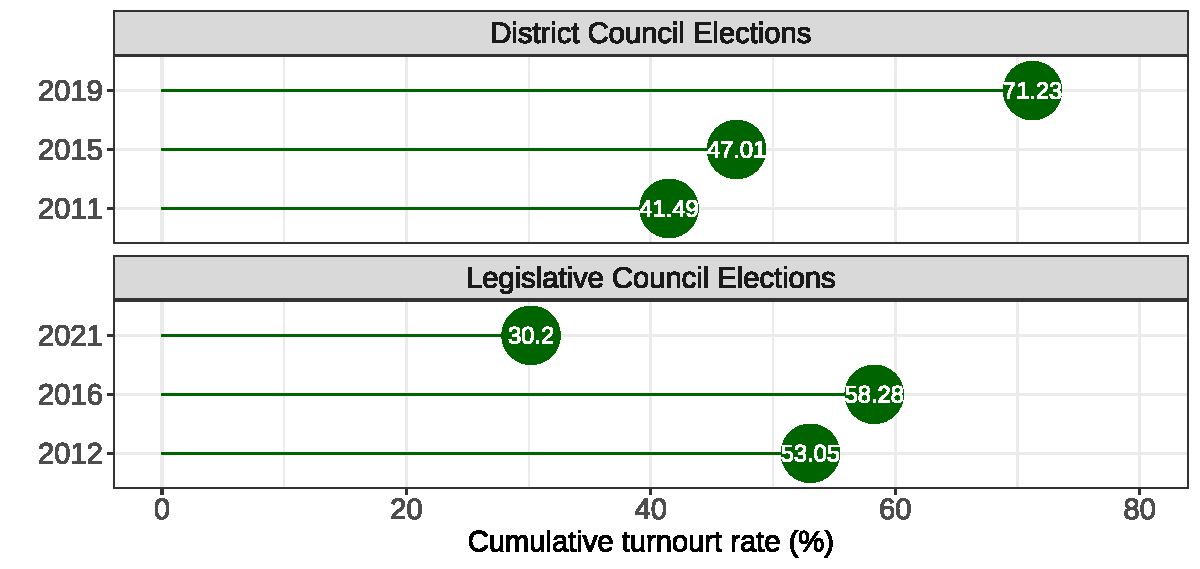
\includegraphics[scale=0.7]{Visuals/trend_turnouts.pdf} 
        \caption{The cumulative turnout rates of elections in Hong Kong, 2011-2021. (Source: the Government of HKSAR)}
        \label{fig: turnouts_trend}
\end{center}
\end{figure}

Mass political consumerism like the Yellow Economic Circle constitutes a key yet understudied form of political dissent during a social movement. Political consumerism is defined as consumers' active use of ``the market as their arena for politics'' (Stolle and Micheletti 2013, \mbox{i}). In general, political consumerism takes form of boycotting and ``buycotting'' (Copeland and Boulianne 2022; Kam and Deichert 2020). During a boycott, politically aware consumers intentionally avoid products because their producers act against the causes those consumers embrace (Bostr{\"o}m 2019). For example, some U.S. consumers have been boycotting Chick-fil-A for its CEO's openly anti-LGBTQ remarks in 2012. On the other hand, consumers sometimes ``buycott'' (deliberately purchase) products produced by firms with practices that are in alignment with their political causes. ``Buycotts'' organized by the anti-LGBTQ community following Chick-fil-A's incident were associated with a 14\% increase in the company's financial revenue (Kam and Deichert 2020). 

Scholars often frame political consumerism as a proxy for consumers' ideological beliefs. Citizens signal their political preferences and reinforce their identities when they decide to ``buycott'' or boycott. Given that political consumerism campaigns sometimes take place within an electoral cycle, two questions arise: Does political consumerism shape citizens' voting behavior? And do mass boycotts and ``buycotts'' increase vote shares for candidates whose ideology is in alignment with the political causes consumers support? 



My research intends to answer these questions using Hong Kong's Yellow Economic Circle during the 2019 Anti-ELAB Movement as a test case of mass political consumerism campaigns under democratic backsliding. It is possible that political consumerism increases turnouts and vote shares for candidates whose political ideologies align with the causes espoused by politically aware consumers through persuasion and mobilization. 

The high turnout rate and remarkable victory for pro-democracy candidates during the 2019 District Council Election surprised many people (Griffiths et al.\ 2019). Previous literature suggests that amid an anti-authoritarian movement, citizens tend to falsify their political support for the authoritarian regime to avoid repression (Goldstone 2001; Kuran 1991; Thelen 1999). But some citizens may also take several small-scale actions that eventually accumulate to unexpected anti-authoritarian political outcomes (Kuran 1991). Political consumerism campaigns are a part of those ``small-scale'' actions, as compared to sit-in protests. On the one hand, dining at restaurants endorsed by the Yellow Economic Circle allows pro-democracy citizens to conceal their true political preferences: They can frame their support for pro-democracy businesses as a quotidian decision---choosing a place to eat---and thus avoid repression from the authoritarian government (Kuran 1991). On the other hand, those political consumerism campaigns convince pro-democracy voters that the cost of supporting pro-democracy candidates may be low. Citizens can have conversations and infer the degree of opposition among other citizens while dining out, which results in a ``bandwagon'' effect that empowers them to get out to vote and reveal their true preferences at the polling stations (Acemoglu et al.\ 2018; Kuran 1991; Wang and Wong 2021; Yanagizawa-Drott 2014).

In the meantime, political consumerism campaigns mobilize a group of consumers by informing them about this local, relatively low-stakes election as many restaurants started encouraging people to register to vote (Arceneaux and Nickerson 2009; Green et al.\ 2016). Political consumerism---manifested in daily consumption decisions---allows both pro-democracy businesses and citizens to signal and reinforce their democratic values (Edmond 2013). Therefore, in the context of democratic erosion in an autocracy, political consumerism may serve as an instrument for citizens to effectively resist government-led democratic erosion by bolstering pro-democracy candidates. 

To empirically measure political consumerism in Hong Kong, I use data from OpenRice \footnote{\url{https://www.openrice.com/en/hongkong}}, the most popular local food service platform where pro-democracy citizens have systematically categorized the political ideologies of thousands of restaurants. Figure \ref{fig: heatmap}, the heatmap, visualizes the proportion of restaurants by their political ideology in each of the 18 large administrative districts of Hong Kong. Different geographical distributions of restaurants with different political ideologies suggest that citizens' exposure to the ideal of the Yellow Economic Circle and its encompassed democratic values may be different (Figure \ref{fig: heatmap}). This might have led to different election outcomes across those constituencies.

Using both politicized restaurant and election data in Hong Kong, I implement a difference-in-differences model with two-way fixed effects to study whether spatial proximity to ``Yellow'' restaurants affects general turnouts and election outcomes for pro-democracy candidates. My empirical analysis reached no statistically significant finding about the electoral impact of the Yellow Economic Circle. Several robustness checks are conducted, and the results consistently indicate no significant effect. The Yellow Economic Circle did not generate a significant impact on either voter turnouts or vote shares for pro-democracy candidates, as some citizens might not take formal politics into consideration when making consumption decisions. Furthermore, it is difficult for the Yellow Economic Circle to sway many voters who are not pro-democracy. This is partly due to the prevalence of local community-based businesses (\begin{CJK*}{UTF8}{bkai}``街坊生意''\end{CJK*}) in this densely populated city. Many Hong Kong citizens already have prior knowledge of their neighbors' political preferences, including those of restaurant owners who frequently host them.

My research aims to bring the existing literature on political consumerism and democratic backsliding into conversation with one another. First, I add a case of mass political consumerism taking place in a hybrid regime under democratic erosion and analyze the electoral consequences of this social movement. Most of the current research on political consumerism has focused on established democracies such as the U.S. and the U.K. (e.g.\ Hainmueller et al.\ 2015; Kam and Deichert 2020; Kyroglou and Henn 2022; Prasad et al.\ 2004; Simon 2011). Yet, there has been limited empirical research on political consumerism in non-democracies and how this type of social phenomenon affects the democratization process in those countries.

Second, my research explores an important topic in democratic backsliding: whether social movements alone can impose checks upon autocrats. More specifically, I test whether pro-democracy political consumerism initiated by private businesses and citizens can effectively resist government-led democratic erosion by exposing voters to the ideology of democratic governance, shaping their voting behavior, and eventually bolstering pro-democracy candidates in elections (Dahl 1971; Downs 1957; Gamboa 2017; Haggard and Kaufman 2021; Hyde 2020).


For the rest of this thesis, I offer an overview of the current research on both political consumerism and democratic backsliding. Following that, I conceptualize the official formation of the Yellow Economic Circle and propose a theory of how it promotes vote shares for pro-democracy candidates and turnouts through persuasion and mobilization. I also set up the hypotheses to investigate the YEC's downstream effects on election outcomes. Next, I detail my research design, which includes an innovative method to observe vote shares in largely coterminous political constituency districts spanning three election years and analyzes the electoral impact of the Yellow Economic Circle with a large novel data set. I then discuss the null results obtained from both my main difference-in-differences models and robustness checks. I also offer several possible reasons for those insignificant results regarding the YEC's electoral impact. Lastly, I discuss how future research, in particular experimental methods, can have the potential to address the inherent deficiencies of observational works like this.



\begin{figure}[!h]
    \centering
    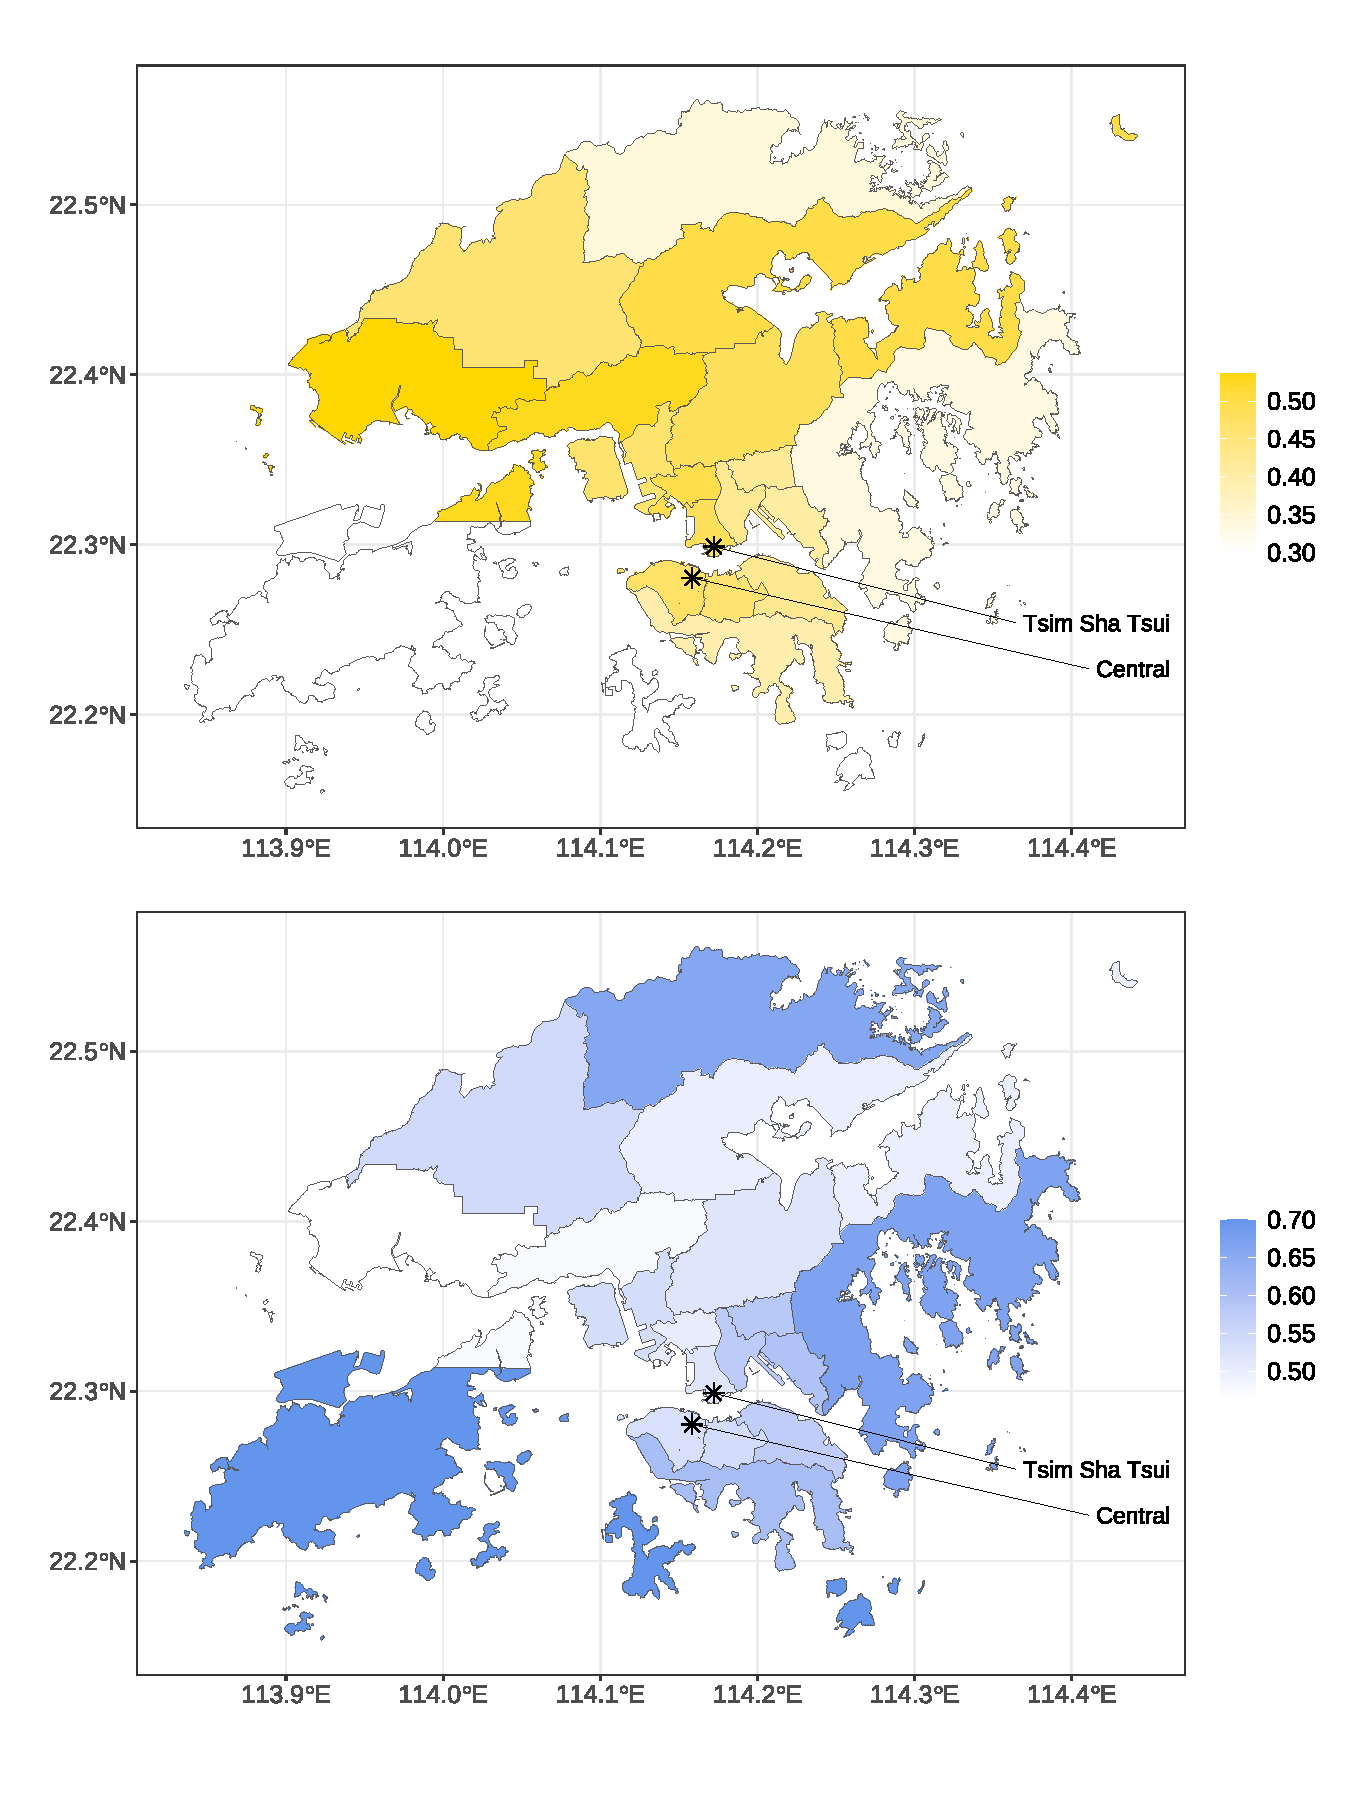
\includegraphics[width=15cm, height=19.5cm]{Visuals/heatmap.pdf}
     \caption{Proportions of ``Yellow (pro-democracy)'' and ``Blue (pro-Beijing)'' restaurants in the 18 large administrative districts. ($n = 2712$. Source: OpenRice)}
    \label{fig: heatmap}
    \floatfoot{\textbf{Notes}: The two stars denote the centroids of two important political and business centers in Hong Kong: Central (\begin{CJK*}{UTF8}{bkai}中環\end{CJK*}; also known as the Central District) and Tsim Sha Tsui (\begin{CJK*}{UTF8}{bkai}尖沙咀\end{CJK*}).}
\end{figure}




%-------------------------------Lit Review
\pagebreak
\section{Existing Literature}
 
\subsection{Political Consumerism}
Social science research on political consumerism typically focuses on consumption at both individual and national levels. I categorize major research on political consumerism at the individual consumption level into two strands. The first strand comes from the economics literature on how price-sensitive politically aware consumers are when they make consumption decisions, knowing the ideological preferences of the producers. Another strand lies in political psychology and investigates the psychological motivations behind boycotts and ``buycotts.'' In addition to focusing on individual consumption, political scientists have long studied economic sanctions imposed by countries and intergovernmental organizations to promote democratization in the sanctioned states.

\subsubsection{At Individual Levels}
Prior economics research on price sensitivity has shown empirically that consumers are politically aware when evaluating the practices of private businesses. Practices that run counter to basic human rights have received the most attention. Those include running sweatshops and exploiting child labor and the environment in less economically developed countries. Those practices usually induce brand rejections and embracing (Bostr{\"o}m 2019). That is, when choosing among brands, some consumers punish certain brands involved in practices against their political causes by withdrawing consumption (Bostr{\"o}m 2019; Kam and Deichert 2020; Sen et al.\ 2001). In contrast, they may reward some producers by intentionally purchasing their products, such as those produced under positive working environments (Bostr{\"o}m 2019; Kam and Deichert 2020; Sen et al.\ 2001).

This strand of literature on political consumerism often adopts experimental methods. It has reached several empirical conclusions regarding consumers' willingness to pay higher prices for products made by companies whose practices are in alignment with their political beliefs. Those studies demonstrate that consumers are indeed considering this alignment when making purchasing decisions. Prasad et al.\ (2004) used a randomized field experiment to show that U.S. consumers respond to politicized labels of brands, such as those certifying that their products are produced under good working conditions. However, consumers might still choose a brand with practices against their values for lower prices (Prasad et al.\ 2004). Moreover, some research in this strand argues that politicized consumption is consumers' way to shape corporate behavior from the demand side. Hainmueller et al.\ (2015) conducted a field experiment in the U.S. to measure the effects of fair trade labels on consumer demand for coffee. They find that even though consumers overall support fair trade products, some price-sensitive consumers will not be willing to pay a high premium. However, the heterogeneity they find in consumers' willingness to pay a high premium requires further research into their decision-making process (Hainmueller et al.\ 2015).

This motivates the second strand of work that largely focuses on understanding the psychological motivations behind political consumerism. Some scholars have studied how social pressure affects consumers' decisions to boycott. Major theories in this line of research draw from social dilemmas and reference groups. Social dilemmas describe the situation in which an individual politically aware consumer has to make a trade-off between their own interest and that of the group when it comes to supporting a political cause (Klein et al.\ 2004; Sen et al.\ 2001). Reference group theory argues that social pressure posed by the group affects consumers' decision to boycott. Sen et al.\ (2001) used two randomized controlled trials to test both theories and conclude that consumers' demand for the boycotted products and their access to substitutes affect their ultimate decision to boycott. Furthermore, prior research also looks into the differences between the motivations behind boycotts and ``buycotts.'' Kam and Deichert (2020) conclude from their experimental results that negative information about the targeted private institutions has more power over inducing boycotting than over inducing ``buycotting.''


However, previous research has typically studied developed democracies, where the targets of boycotts and ``buycotts'' are private institutions only. In those cases, individual consumers do not expect the government to take action to influence corporations or to generate far-reaching political changes (Kam and Deichert 2020; Simon 2011). There is a clear boundary between private institutions and the government. Existing studies thus treat political consumerism as a single mode of political participation, even though they frequently frame it as a proxy for the ideological identities or preferences of consumers (Simon 2011; Stolle and Micheletti 2013). 

\subsubsection{At National Levels}
Although political consumerism at times occurs within the temporal proximity to elections, few scholars have looked into the actual political impact of political consumerism, especially how individual consumption affects the political outcomes within a country. Most research that has attempted to make the connection between political consumerism and its political impact is focused on a cross-national level. The most frequently studied type of cross-national political consumerism is economic sanctions imposed by a country or an inter-governmental organization on another country. Those studies have reached mixed conclusions about the effectiveness of economic sanctions on democratization in sanctioned countries (Grossman et al.\ 2018; Wood 2008). Examples include boycotts against products from South Africa issued by the United Nations to support the anti-apartheid movement (Schwartzman 2001), the European Union labeling products from Israeli settlements (Grossman et al.\ 2018), and the U.S. embargo against Cuba (Schwartzman 2001; Wood 2008). 

Grossman et al.\ (2018) were among the first that used a survey experiment to study the effect of international economic sanctions on the targeted population. As a part of their experiment, they investigated if being exposed to information about the EU labeling products from Israeli settlements affects voting behavior. They find that the exposure to such information decreases support for the incumbent Prime Minister Benjamin Netanyahu, who favored hawkish policies in response to the sanctions (Grossman et al.\ 2018). Even though the boycotts against Israeli products were initiated outside the country, the fact that political consumerism is able to shape voters' choices sheds light on the possibility that mass and effective campaigns may persuade and mobilize consumers to vote for candidates whose political preferences are in alignment with the political ideology behind those campaigns.

By connecting political ideological preferences exhibited in broad-based political consumerism to citizens' voting behavior, it is possible to test a newly emerging topic in the broad literature of democratic backsliding: Are movements supported by private businesses able to promote effective resistance against elite-led democratic erosion? In the case of Hong Kong, a hybrid regime, I define citizens' resistance as voting for pro-democracy candidates and test whether mass political consumerism benefits the opposition parties and candidates by increasing their vote shares (Gamboa 2017; Wang and Wong 2021).


\subsection{Democratic Backsliding}
While the concept of democratic backsliding is relatively new, it relates to a long-standing literature in political science. Many scholarly works on democratic backsliding are built on larger bodies of literature such as political institutions, democratization, and regime changes. Notably, Bermeo (2016) distinguishes six types of democratic backsliding. Using global cases after the Cold War, Bermeo (2016) argues that while there has been a decreasing trend in some types of backsliding such as classic coups, executive coups, and election-day fraud, other types such as promissory coups have remained unchanged or even been increasing. Nonetheless, current research on democratic backsliding has reached a consensus that it has been a gradual process rather than sudden (Bermeo 2016; Haggard and Kaufman 2021; Hyde 2020). In some contemporary cases, democratic backsliding even received popular support (Hyde 2020). That being said, backsliding has been endorsed by a large proportion of supporters of the state actors who initiated democratic backsliding (Bermeo 2016). A recent example of this is social movements in Thailand between 2013 and 2014 that supported the removal of the lawfully elected Prime Minister, Yingluck Shinawatra, from office. The fact that backsliding is slow and elicits popular responses suggests that well-organized election campaigns while backsliding is happening may be effective in preventing further erosion.

\vspace{6pt}

\begin{figure}[h!]
\begin{center}
        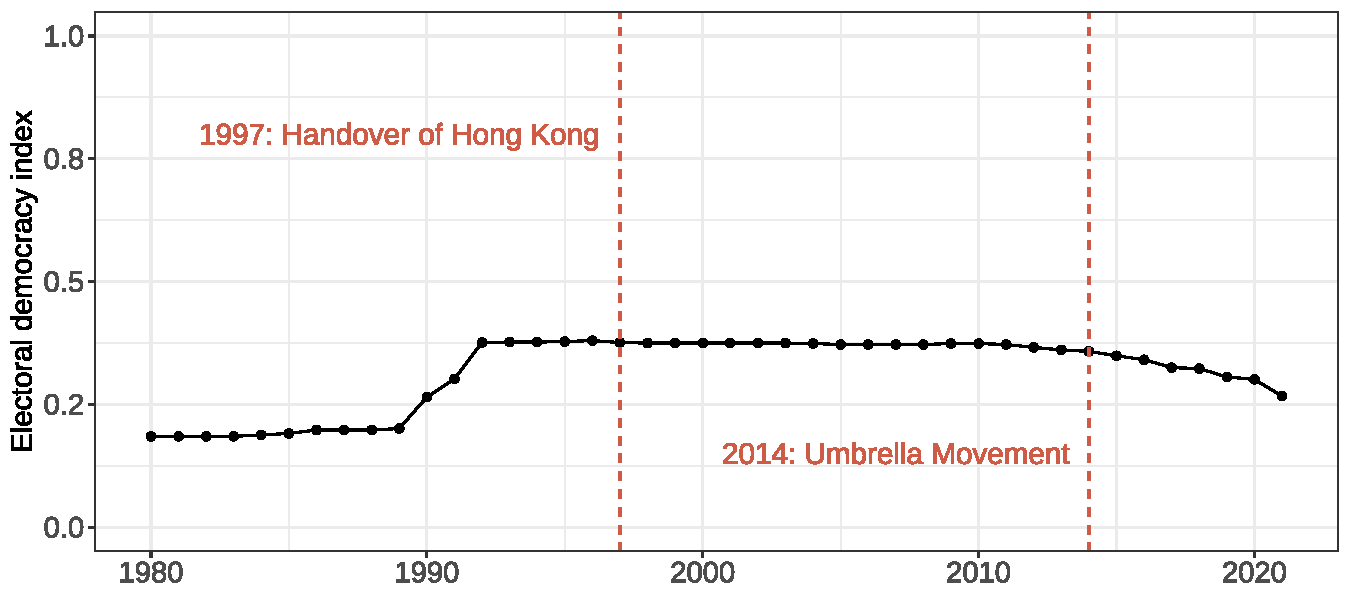
\includegraphics[scale=0.7]{Visuals/vdem.pdf}
        \caption{Electoral Democracy Index [0-1] of Hong Kong, 1980-2021 (Source: Varieties of Democracy (V-Dem))}
        \floatfoot{\textbf{Notes}: The figure shows an expert-coded index that evaluates measures of democracy such as universal suffrage and freedom of speech. The variable is named ``v2x\_polyarchy'' in the original V-Dem data set.}
        \label{fig: vdem}
\end{center}
\end{figure}



\subsubsection{Democratization and De-Democratization in Hong Kong}

Indeed, Hong Kong's democratization or de-democratization process may differ from the mainstream democratic backsliding theory that often cites established democracies. This is partly because Hong Kong was a former British colony that had never enjoyed a full democracy before and after 1997. It had not been a part of the wave of Post-World War \mbox{II} decolonization, featured by political regime transitions from autocracies to democracies (Darwin 1997). Although there might have been an increase in its democratic features after the U.K. government transferred its sovereignty back to the People's Republic of China, Hong Kong did not experience drastic institutional changes (Darwin 1997). As Haggard (1990, 155) points out, the British government facilitated the implementation of certain limited democratic features, including preserving some degree of political autonomy in Hong Kong (e.g.\ elections), only for both ``ideological and practical reasons'' before the issue of the Joint Declaration.

However, democratic erosion initiated by the Chinese Communist Party (CCP) after the handover features the characteristics summarized by the current research on democratic backsliding. It has been an incremental process rather than a shock. According to the Electoral Democracy Index coded by the Varieties of Democracy Project (2022), there has been a gradual decrease in the degree of political rights Hong Kong citizens can exercise, such as having responsive officials and freedom of association since 2014, the year when the Umbrella Movement took place (Figure \ref{fig: vdem}). Furthermore, the case of Hong Kong is consistent with Bermeo's argument that some state-led democratic erosion receives support from citizens. A decent proportion of Hong Kong citizens support the pro-Beijing government or the mainland government as a whole (Xinhua News Agency 2019). Research on such a complex case will enable a nuanced understanding on top of the current theory of democratic backsliding.



\paragraph{Authoritarian Elections as Power Sharing} 
To understand the complexities induced by Hong Kong being a hybrid regime, it is important to take a step back and discuss whether the region's democratization or de-democratization process before and after the handover in 1997 is explained by existing literature. More importantly, why, in the very first place, did the authoritarian central government in Beijing agree to allow for competitive elections in Hong Kong? And more fundamentally, why did the ruling autocrats in Beijing allow for party institutionalization and different political ideologies among voters?

Current institutional theory on power sharing suggests some rationales for authoritarian elections in Hong Kong. Geddes (1999; 2005) points out that elections---even competitive ones---are not uncommon in autocracies, even though the purpose of those elections may differ from that of those in democracies. Boix and Svolik (2013) argue that autocrats allow for elections because doing so allows them to come into power. They understand that elections may be the only way for them to remain in power, but in the case of Hong Kong, to remain in power requires the autocrats to acquire power first (Boix and Svolik 2013; Wong 2015). 

The constitutional design of Hong Kong as a Special Administration Region was not an easy task for the CCP during their negotiations with the British government. One of the most daunting hurdles was that the CCP needed to address the ideological diversity that already existed in the region while sustaining Hong Kong's economic stability and future development. Historically, Hong Kong had harbored refugees who fled the mainland China due to political persecution and different political stances (Wong 2015). 

Moreover, by the time the negotiations began, Hong Kong had become one of the world's most preeminent financial centers on par with Singapore and Japan. Strategically, sustaining Hong Kong's economy would ensure continual inward foreign direct investment and in turn benefit the ongoing economic reform in the mainland China (Haggard 1990). Many citizens had decided to immigrate to the U.K., the U.S., and Canada before the handover, showing concerns for Hong Kong's future democratic development. Prior research suggests that such emigration waves led to a shortage of labor and impacted Hong Kong's economy (S. Wong 1992). The ruling elites in Beijing had to preserve some degree of political autonomy to reduce this impact of population sorting and ensure that citizens in Hong Kong would not subvert the new government due to drastic changes in its political and economic institutions. 

However, the ruling elites did not promise that they would keep this autonomy forever. There are several ambiguities and uncertainties in Hong Kong's ``one-country, two systems (\begin{CJK*}{UTF8}{bkai}一國兩制\end{CJK*})'' constitutional principles. Scholars have not yet agreed upon whether these ambiguities were inherited from the fact that the principles have been a completely new design in practice, or they were Beijing's tactics to renege in the future if necessary. Therefore, those ambiguities and uncertainties produce concerns for both the autocrats and citizens regarding Hong Kong's political future.

\paragraph{Authoritarian Elections as Control Mechanisms} 
Nevertheless, uncertainties brought by the constitutional design in Hong Kong did not rule out the opportunities for Beijing to still have control over the region under power sharing. Svolik's (2012) coalition theory offers an explanation for one of the control measures: If Beijing appears to be politically powerful enough, it is extremely difficult for the existing ruling coalition to separate itself from the central government (Svolik 2012). In this case, Beijing has formed long-term coalitions with the pro-establishment parties in Hong Kong. Those parties have long framed Beijing's ruling as a decolonization effort and the warrant for a promising economic prospect. In the meantime, those coalitions also run campaigns to showcase their invincibility and attract more allies and supporters (Svolik 2012).

Furthermore, because those pro-establishment parties are dominated by business elites in Hong Kong, clientelism and loyal political party machines have become another one of Beijing's control mechanisms (Blaydes 2010; Haggard 1990; Stokes 2005). For example, following theories of political clientelism (Stokes 2005), it is theoretically possible for Beijing to have loyal local party machines mobilize voters for them, such as those pro-establishment/pro-Beijing parties. That being said, those parties are able to infer voters' preferences given that Hong Kong is one of the most densely populated cities in the world with a very limited living environment (Blaydes 2010; Stokes 2005). 


% table
\newcolumntype{C}{>{\RaggedRight\arraybackslash}X}
\begin{table}[h!]
\fontsize{11}{12}\selectfont
\setlength\extrarowheight{2pt} % for a bit of visual "breathing space"
\begin{tabularx}{\textwidth}{||CCCC||}
\hline
\textbf{Time Period} & \textbf{Event} & \textbf{Immediate Goal} & \textbf{Underlying Goal}  \\
\hline \hline
2011-2012 & The Occupy Central Movement & To support the Occupy Wall Street Movement in New York City & To protest against economic inequality in Hong Kong \\
\hline
2014-2015 & The Umbrella Movement & To oppose Beijing's move to pre-approve candidates for the Chief Executive & To call for free elections and universal suffrage (``one person, one vote'') \\
\hline
July 1, 2016 & The July 1 March & To condemn the current Beijing-endorsed Chief of Executive (Leung Chun-Ying) & To encourage local parties to run for the 2016 Legislative Council Election and continue calling for universal suffrage \\
\hline
2019-2020 & The Anti-Extradition Law Amendment Bill Movement & To stop the enactment of the bill  & To continue calling for universal suffrage and preserve Hong Kong's political autonomy\\
\hline
\end{tabularx}
\caption{List of anti-authoritarian movements in Hong Kong, 2010-2020. (Sources: Cantoni et al.\ 2019, Wong 2015, and online news)}
\label{tab:movements}
\end{table}

\paragraph{Anti-Authoritarian Movements}

The Joint Declaration states that Hong Kong will enjoy political autonomy---which was also signed into its Basic Law---for 50 years (Constitutional and Mainland Affairs Bureau 2007; Martin 2010). However, it doesn't state what will happen if Beijing reneges and whether Hong Kong will become a full democracy under the ``50-year promise.'' Hong Kong's restricted autonomy is therefore conditional on whether Beijing is willing to be a lenient autocrat (Wong 2015). While pro-democracy citizens use the inherent ambiguities in the design of ``one country, two systems'' to preserve or advocate for more political rights such as universal suffrage and free and fair elections, Beijing uses the same ambiguities to suppress their causes (Cantoni et al.\ 2019; Martin 2010). 

Consequently, the 2010s in Hong Kong witnessed several mass anti-authoritarian movements (Table \ref{tab:movements}). The government of HKSAR and the central government in Beijing have led pro-democracy citizens in Hong Kong to believe that democratization has ended in Hong Kong through its acts across the years (Wong 2015). Beijing proposed to pre-approve candidates for the Chief Executive in 2014 (Table \ref{tab:movements}, Row 2). In 2019, the government of HKSAR proposed a bill that includes the mainland China as one of its extradition destinations and raises serious concerns about Hong Kong's judicial independence (Leung 2019). Moreover, the enactment of the National Security Law in 2020 has furthered this belief by crushing the possibility of anti-authoritarian protests. When state-led repression constantly occurred and had been followed by the legitimate lockdown during the COVID-19 pandemic, pro-democracy citizens had to diversify their protest strategies while mobilizing more people to join their campaigns.

This is an extremely difficult task. Existing literature on anti-authoritarian movements suggests that under state-led repression, citizens may falsify their true political preferences for practical reasons (Kuran 1991; Thelen 1999). Kuran (1991) has identified the distinction between private preferences and public preferences: The former is usually fixed but not shared with others, while the latter is variable since a citizen can choose how they want to appear in public. When a citizen's private preference differs from their public one, they are falsifying (Kuran 1991). Therefore, political dissent alone does not effectively mobilize people to participate in social movements (Kuran 1991). The opposition groups have to consider various resources they can utilize to challenge the autocratic incumbents while true preferences are not shared and thus true public preferences are difficult to gauge (Haggard and Kaufman 2016). 

Mass political consumerism has the potential to address the issue of private preferences not being shared and the cost of joining the anti-authoritarian movements when citizens coordinate election campaigns for candidates whose political ideologies align with theirs. Although the Chinese government has demonstrated its ability to slow down the spread of information for protesters to organize demonstrations in the streets (King et al.\ 2013), they may not micromanage individual consumption decisions (in the case of Hong Kong, where to eat). The perceived cost of participating in pro-democracy political consumerism is relatively lower than taking it to the streets, as citizens can frame their participation as a simple daily decision. As elections approach, citizens may be able to infer others' preferences by observing other citizens make the same consumption decisions at restaurants that send clear political signals. Those observations, which consolidate a group identity, may stimulate critical pushback at polling stations (Goldstone 2001; Kuran 1991). 


%-------------------------------Theory

\section{Conceptualizing the Case of Hong Kong}
\begin{figure}[h!]
\centering
        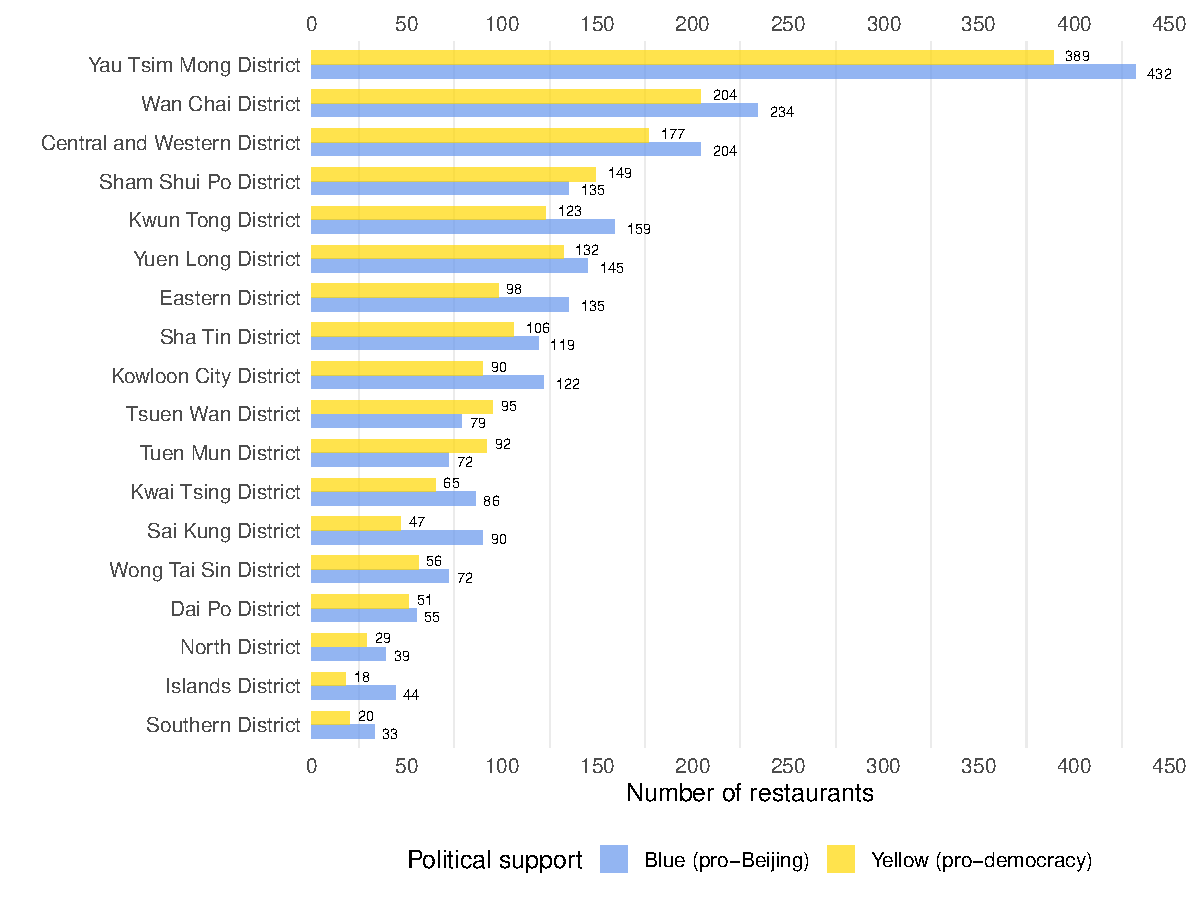
\includegraphics[scale=0.8]{Visuals/bar_restaurant_by_district.pdf} 
        \caption{Numbers of restaurants in each of the 18 administrative district by political support. ($n = 4196$ (full sample). Source: OpenRice.)}
        \label{fig: openrice}
\end{figure}

\subsection{The Formation of the Yellow Economic Circle}
The formation of the Yellow Economic Circle (YEC) was reactive at its beginning. Yoshinoya (\begin{CJK*}{UTF8}{bkai}吉野家\end{CJK*}) is a Japanese multinational fast food company that owns 35 restaurants in Hong Kong. After four months into the 2019 Anti-ELAB Movement that officially began in March, Yoshinoya fired one of its staff for their opposition to the proposed extradition bill (Su and Cheung 2019). Yoshinoya's decision outraged many pro-democracy protesters, who view their act as pandering to an authoritarian government. Later, pro-democracy protesters organized boycotts against all Yoshinoya restaurants in Hong Kong (Su and Cheung 2019). This marked the inception of the official formation of the YEC. 

The YEC continued to develop as protests expanded to almost all administrative districts of Hong Kong (Figure \ref{fig: openrice}). To date, the YEC has become systematic and economically high stakes. Pro-democracy protesters created their own typology of restaurants based on their political preferences during the protests (Appendix \ref{appendix:categorization_system}). They divided restaurants into two political ideological groups: ``Yellow'' represents those operated by pro-democracy owners or offering free meals to protesters. ``Blue'' denotes those with owners or operators who support the pro-Beijing government and denounce the protests. Among those ``Blue'' restaurant owners, many are companies that have financial ties with big corporations in the mainland. After state-led repression occurred and had been constantly threatened, protesters organized ``buycotts'' by advocating dining at ``Yellow'' restaurants and boycotts against ``Blue'' ones to diversify their protest strategies. 

Both business owners and pro-democracy citizens have made collective efforts to gather information about restaurants' political preferences. Some restaurants actively signaled their preferences by putting up posters. An example in Appendix \ref{appendix:yellow_sticker_slogan} shows the most frequently used poster for pro-democracy restaurants, which includes the most popular slogan for the Anti-ELAB Movement: ``Liberate Hong Kong, revolution of our time (\begin{CJK*}{UTF8}{bkai}``光復香港,時代革命''\end{CJK*}).'' Another example in Appendix \ref{appendix:yellow_sticker_slogan} demonstrates the cooperation between pro-democracy business owners and citizens: They imitated the practice of the MICHELIN guide by putting up a sticker on the outside of a pro-democracy restaurant. Pro-democracy citizens also posted their own observations about restaurant owners' political support amid the protests on social media platforms (Appendix \ref{appendix:openrice_usercomments}). To offer information shortcuts and coordinate this campaign of political consumerism, some pro-democracy protesters set up accounts on OpenRice, Hong Kong's most popular food service platform.

In addition to being systematic, the YEC is also economically high-stakes. Ranging from MICHELIN-starred fine dining restaurants to open-air food stalls (``Dai Pai Dong''), Hong Kong's diverse food service industry has been key to its tourism, the second largest pillar industry of Hong Kong's economy. According to a report by the United States Department of Agriculture (USDA) in 2020, the city hosts more than 16,000 restaurants, with approximately 2158 restaurants per 10,000 people on average. A Bloomberg article in 2020 estimated that the market value of the Yellow Economic Circle alone had reached approximately 12.9 billion U.S. Dollars (Prasso 2020). 


\vspace{9pt}
\begin{figure}[h!]
\begin{center}
        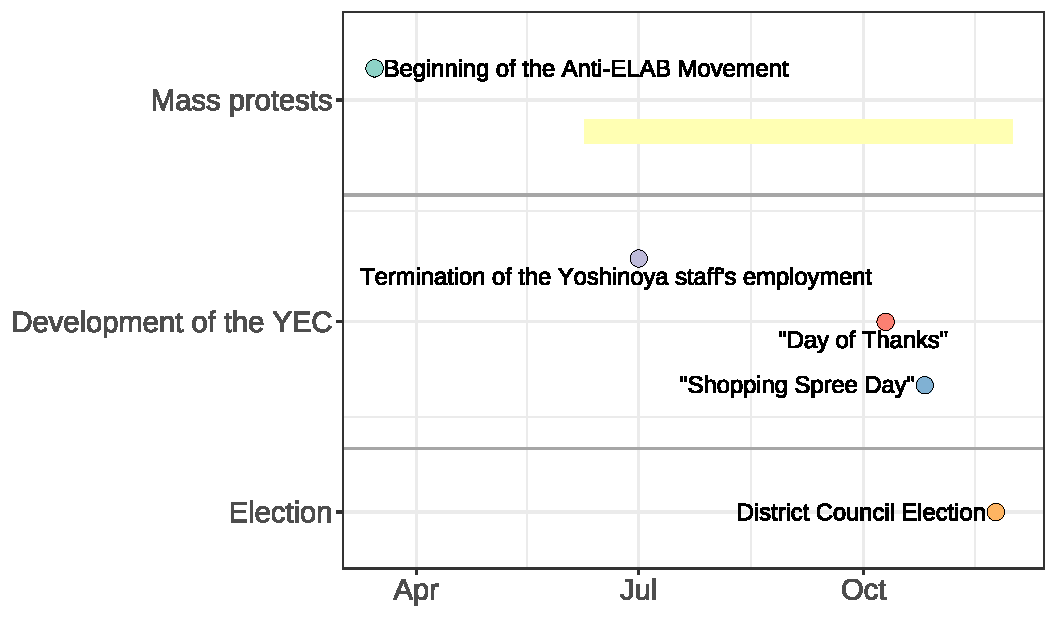
\includegraphics[width=15cm, height=9cm]{Visuals/timeline_yec.pdf} 
        \caption{The timeline of the development of the YEC (March 2019 - December 2019).}
        \label{fig: timeline}
\end{center}
\end{figure}


The reasoning behind this pro-democracy political consumerism is simple. People in Hong Kong---the city with such a high density of restaurants in the world---usually dine out due to the limitations of their work and living environment (USDA 2020). For both pro-democracy protesters and business owners, the YEC fits well with their immediate and long-term political goals. In the short run, some pro-democracy protesters value the political ideological labels of restaurants, given that protests in 2019 often took place during lunch hours and in city centers (Figure \ref{fig: protests}). The official implementation of the National Security Law in June 2020 has made massive gatherings and marches impossible under the law for pro-democracy protesters. Not only did the National Security Law mark the elite-led democratic erosion of Hong Kong's rule of law and civil liberties, but it also forces pro-democracy protesters to come up with new strategies to avoid repression (Bermeo 2016; Hyde 2020). This is when broad-based political consumerism has become an important social movement as participating in it can be seen as apolitical quotidian decisions (Kuran 1991). 

\vspace{9pt}
\begin{figure}[h!]
\begin{center}
        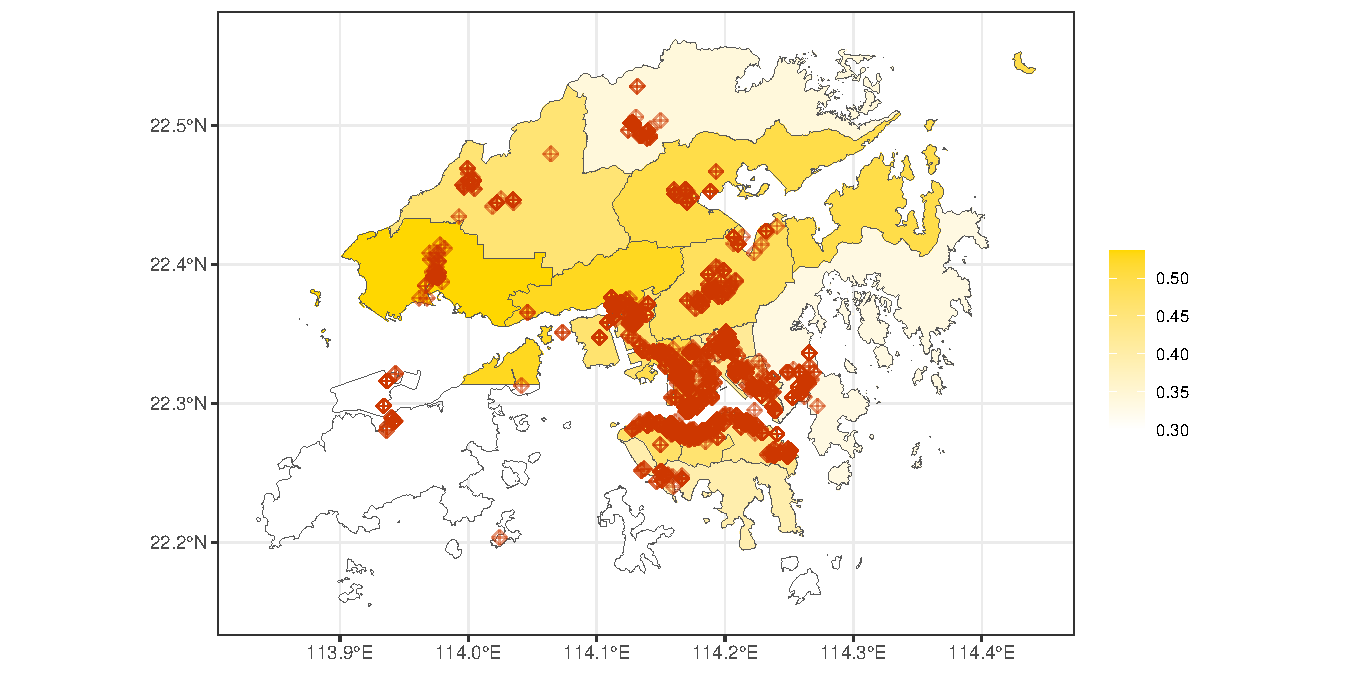
\includegraphics[scale=0.8]{Visuals/protest-sites.pdf} 
        \caption{Protest sites during the 2019 Anti-ELAB movement mapped onto the heatmap of the proportions of ``Yellow'' restaurants in 18 large administrative districts. (Sources: HKU and Openrice)}
        \floatfoot{\textbf{Notes}: Each red marker represents a protest between June 12 and December 31, 2019. Those include sit-in protests, marches, Lennon Wall(s), screening of videos in which pro-Beijing protesters attacked pro-democracy protesters (Teo and Fu 2021).}
        \label{fig: protests}
\end{center}
\end{figure}


In the long run, protesters believe that achieving economic independence is key to resisting both the economic and political pressure from the central government in Beijing (Wong et al.\ 2021). Haggard (1990) gives historical evidence that Hong Kong's legislative institutions are dominated by business elites. Forming an economic circle to support like-minded local businesses and punish the pro-Beijing counterparts has therefore become their first step to shaping elite behavior. This also highlights a difference between existing research on political consumerism: in this case, politically aware consumers intend to shape governmental behavior by boycotting business elites (Acemoglu et al.\ 2018; Poon and Tse 2022; Wong et al.\ 2021).






\subsection{Mechanisms for Electoral Consequences}
The Yellow Economic Circle has continued to expand both temporally and spatially since its official inception in July 2019. It experienced a local election in Hong Kong and reached all constituency districts (Figures \ref{fig: openrice} and \ref{fig: timeline}). Notably, before the 2019 District Council Election in November, pro-democracy protesters organized two mass ``buycotts'' to show their gratitude to the ``Yellow'' restaurants that supported the protests and offered free meals to pro-democracy protesters (Figure \ref{fig: timeline}). The 2019 District Council Election recorded the highest turnout in Hong Kong's electoral history and a remarkable victory for pro-democracy candidates and protesters (Figure \ref{fig: turnouts_trend}). I hypothesize that the YEC may have generated electoral consequences through two major mechanisms: persuasion and mobilization.


\subsubsection{Why Institutional Strategies}
Before I dive into explaining the two mechanisms, there is still, however, a question remaining: Why did pro-democracy citizens still rely on elections, an institutional strategy, to resist democratic erosion? Political scientists give three reasons in general:
\begin{enumerate}
    \item First and foremost, non-institutional strategies, characterized by physical violence, are extremely risky and costly (Dunning 2011). The 1989 Tiananmen Square massacre demonstrates Beijing's history of repression of political dissidents. Given that Beijing has stationed the People's Liberation Army in Hong Kong, it is safer for protesters to adopt an institutional strategy when it is still available.
    
    \item For both pro-democracy candidates and protesters, winning elections grants them legitimacy within the political regime and the international community (Gamboa 2017). Many saw this low-stakes election amid protests as an opportunity to poll popular support for both pro-democracy and pro-Beijing groups (Griffiths 2019). While international support for Hong Kong, particularly sanctions on its officials imposed by the U.S. and the U.K., was weak (Hyde 2020), gaining legitimacy through an election might give the international community the grounds to continue pushing for subsequent refugee, asylum, and immigration policies\footnote{Examples of those policies are: (1) The British government under Boris Johnson's leadership set up a visa program with the possibility of turning into citizenship for HK citizens; and (2) The Canadian government allows HK citizens with eligible educational degrees to apply to work in Canada under temporary work permits.} for Hong Kong citizens.
    
    \item Practically speaking, it is still safer for the opposition party (in this case, pro-democracy parties in Hong Kong) to retain some power within the legislature in case of sudden aggressive shocks initiated by autocrats (Gamboa 2017).
\end{enumerate}


\subsubsection{Persuasion and Mobilization}
Did the Yellow Economic Circle play a crucial role in pro-democracy citizens' institutional strategy? I argue that the Yellow Economic Circle helped galvanize support for pro-democracy candidates through two mechanisms: persuasion and mobilization.

The Yellow Economic Circle has the potential to convince citizens who are already pro-democracy to vote for pro-democracy candidates amid mass protests. In reviewing existing literature on authoritarian movements, I argue that Kuran's (1991) theory of preference falsification allows pro-democracy citizens, when living under the threats of state-led repression, to hide their preferences as individual daily consumption decisions may be too trivial to be controlled by the authoritarian central government. However, another part of his theory argues that citizens continue to falsify their preferences even when a revolution begins, which is also why the 2019 election results surprised many in Hong Kong (Edmond 2013; Goldstone 2001; Griffiths 2019; Kuran 1991). 

In the meantime, the Yellow Economic Circle can also persuade and sway voters who are not pro-democracy, as restaurants provide people with spaces to gather, meet new people, and exchange ideas. For example, people talk with each other when dining out. The opportunity to listen to a few outspoken pro-democracy customers' conversations may successfully convince voters on the fence to support pro-democracy candidates. Moreover, those gatherings and conversations allow those undecided voters to gauge the extent of public opposition. There is a threshold for individuals to decide to join the anti-authoritarian movements even though the actual cost of doing so remains high (Goldstone 2001; Kuran 1991). Individual citizens may join the movements when they become certain that public opposition surges, as the punishment may be less severe and the cost of joining the movements is lower than that of hiding their true preferences (e.g.\ sacrifice of their integrity) (Kuran 1991). 

In addition to helping citizens realize the threshold to join a social movement, the Yellow Economic Circle further promotes votes by reinforcing the alignment of the ideology behind those political consumerism campaigns and pro-democracy candidates. Grossman et al.\ (2018) have given empirical evidence that political consumerism campaigns may encourage voters to evaluate the alignment between their political preferences and those of the politicians. In the case of Hong Kong, both pro-democracy candidates and participating business owners in the YEC have used the same slogans to advocate for democratization (see Table \ref{tab:candidate_profiles} and Appendix \ref{appendix:yellow_sticker_slogan}). By reinforcing this alignment of their ideologies, the YEC might have helped canvass more votes for pro-democracy candidates. 

Furthermore, the YEC also mobilized voters who were not likely to vote in a low-stakes election by providing information about the District Council Election. As described in the restaurant categorization system of the YEC, there are some business owners who actively encouraged customers to register to vote (Appendix \ref{appendix:openrice_usercomments}). Again, slogans and stickers put up in ``Yellow'' restaurants resonated with many electoral messages used by pro-democracy candidates (Appendix \ref{appendix:yellow_sticker_slogan}). That being said, those slogans and stickers might have served in the same spirit of those lawn signs during some low-salience U.S. local elections to translate information and therefore encourage voters to get out to vote (Arceneaux and Nickerson 2009;  Green et al.\ 2016). 

\paragraph*{Alternative Mechanism} \label{section:alternative_mechanism}
Given that protests took place concurrently with both the development of the Yellow Economic Circle and the 2019 election, I will also investigate those protests further as an additional mechanism. As mentioned before, some restaurants participating in the YEC demonstrated the core ideals of the Anti-ELAB Movement and offered free meals to pro-democracy protesters. Moreover, some ``Yellow'' restaurant owners allowed their staff to participate in the protests without retaliation and joined the city-wide strikes in October and November (Appendix \ref{appendix:openrice_usercomments}; Chan 2019). It is possible that the YEC also encouraged protests while rallying voters' support for pro-democracy candidates. I will empirically test this alternative mechanism in the results section.


\subsubsection{Hypotheses}
I argue that political consumerism increases the general turnout rate and vote shares for candidates whose political ideologies are in alignment with causes embraced by politically aware consumers through persuasion and mobilization. In the context of democratic backsliding, political consumerism serves as an instrument for politically aware consumers to resist democratic erosion led by the government through electing pro-democracy candidates. If the two major mechanisms provided above are true, I will be able to observe evidence that supports the following hypotheses: 

\begin{itemize}
    \setstretch{1.15}
    \item \bm{$H_{1A}$}: \textit{Spatial proximity to pro-democracy restaurants increases voter turnouts in District Council elections on average.}
    \item \bm{$H_{2A}$}: \textit{Spatial proximity to pro-democracy restaurants increases vote shares for pro-democracy candidates on average.}
    \item \bm{$H_{3A}$}: \textit{Spatial proximity to pro-democracy restaurants decreases vote shares for pro-Beijing candidates on average.}
\end{itemize}




%-------------------------------Methods

\section{Quantitative Methodology}
I use quantitative methods, in particular quasi-experimental methods, to test these hypotheses. Existing research on political consumerism during the 2019 Hong Kong protests relies heavily on qualitative case studies such as interviews and analyzing online platform posts (e.g. Lee and Fong 2021, Poon and Tse 2022, Wong et al.\ 2021). Few have attempted to connect this broad-based social phenomenon to its electoral consequences. While qualitative case studies are helpful to understand and substantiate the incentives of politically aware consumers, establishing the causal relationship between political consumerism and election outcomes requires other methods. An ideal method is a well-designed large randomized controlled trial. However, running a large randomized controlled trial that involves interventions on an autocracy's electoral institution amid protests does not seem to be feasible in the case of Hong Kong (Angrist and Pischke 2009). Therefore, I will detail how I plan to use the difference-in-differences (DiD) identification strategy to analyze the electoral impact of political consumerism in Hong Kong.

\subsection{Data}
To wrangle data for my statistical analysis, I use two data sets: election outcomes at individual polling stations and politicized restaurant data. The District Council Election in Hong Kong adopts a single-member plurality system (``first-past-the-post''). Election results, along with the geographical geometries of District Council constituencies, are published on the government's websites (Appendix \ref{appendix:election_data}). I use data for votes cast at individual polling stations and aggregate them at individual District Council Constituency (DCC) levels for the three District Council elections in 2011, 2015, and 2019\footnote{According to the Government of HKSAR, DCCs were drawn to ensure that each constituency includes a population of roughly 18,000. Note that in all three election years, the polling station at the AsiaWorld–Expo was used for counting misplaced ballots for the 18 large administrative districts. Because this polling station did not observe election outcomes in a specific DCC, those ballots are dropped when I aggregate votes at polling stations to DCCs.}. Note that in 2011 and 2015, there were several uncontested DCCs, where only a single candidate was running and therefore automatically elected (Table \ref{tab:uncontested_by_ideo}). Those candidates thus did not receive a specific number of votes. The issue of those uncontested districts is further addressed in the robustness checks section. 

I also exclude outcomes for both the Chief Executive Elections and the Legislative Council Elections between 2011 and 2022. This is because I intend to study whether YEC mobilizes voters for low-salience local elections. 

As for the politicized restaurant data, I initially collected public information about 4,196 restaurants from OpenRice, Hong Kong's most popular online food service review platform. Specifically, this data set includes names, addresses, and political ideological labels assigned by pro-democracy users for those restaurants \footnote{See Appendix \ref{appendix;full_restaurant} for the codebook and summary statistics of the full restaurant data set.}. I automated this data collection process by writing a webpage scraper in Python. I used Google Maps Geocoding API\footnote{API stands for ``Application Programming Interface.'' The Google Maps Geocoding API serves to automatically retrieve latitude/longitude coordinates using geographical information. See \url{https://tinyurl.com/cdlj889} for more information.} to retrieve the geographical coordinates of each restaurant to later match it to its electoral constituency. Sometimes the API was unable to geocode a restaurant due to its peculiar name or there being multiple locations with the same name. In those cases, I asked the API to set the coordinates for those restaurants to zero. Then I manually inputted geographical coordinates for those cases that Google failed to code. 

To understand how accurately Google's Geocoding API works for those successfully coded cases, I manually audited approximately 10 percent of the restaurants' coordinates ($n = 420$) (Appendix \ref{appendix:audits}). The audited sample was randomly selected. One of the world's most densely populated cities, Hong Kong is packed with high-rise buildings, which oftentimes are large shopping malls that host many restaurants. Google's Geocoding API uses a two-dimensional map that does not show floor plans within a building. As a result, the API sometimes sets the coordinates of certain restaurants to those of the entrances, exits, or parking lots of high-rise buildings. To account for this, I consider the retrieved coordinates to be accurate if they are within 200 meters ($\approx 0.12$ miles) of the actual location of a restaurant's centroid. Google's Geocoding API coded 95.5\% of the restaurants in the audited sample accurately (Appendix \ref{appendix:audits}). I corrected the geographical coordinates for those miscoded restaurants in the audit manually.


\subsection{Defining the Outcomes}
As described in my hypotheses, the outcomes of interest are the turnouts and vote shares for pro-democracy and pro-Beijing candidates at an individual District Council Constituency (DCC) level. However, the redrawing of constituency boundaries prevents me from consistently comparing election outcomes for all individual District Council Constituencies across the three elections. Similarly, added new districts also do not allow me to directly connect the concentration of politicized restaurants to the election result observed in a DCC across years. 

To protect my statistical analysis from those complications induced by redistricting, I follow the methods adopted by prior researchers to address the issue of non-coterminous districts and create a new unit of analysis that is largely consistent across the three election years (Nellis and Siddiqui 2018). To identify the districts with a high degree of stability across three election years, I calculate the percentage of overlapping areas in an individual DCC of a specific year. In my finalized data set, I keep a DCC intact if it met the following two criteria: (1) The DCC remained unchanged for at least 90 percent across three election years; and (2) It was not split from or covered by any other DCCs that underwent changes in areas larger than 10 percent in a given year of the three election years. Then I create ``\textit{joined districts}'' that combine those DCCs that had not met the two criteria by figuring out how they were redistricted in a given year, such as being split from a large district in a previous year (Nellis and Siddiqui 2018, 56)\footnote{I include examples and detailed illustrations of this process in Appendix \ref{appendix:joining_methods}.}. 

This method allows me to observe the election outcomes for 336 joined constituency units that are geographically consistent across three election years. If I were to simply drop those DCCs that underwent significant redistricting (i.e.\ The change of the constituency area was larger than 10 percent between 2011 and 2015 or between 2015 and 2019), I could only observe 205 geographical units. This number would only be approximately half of the district constituency districts in Hong Kong for an election year\footnote{Detailed information about the original numbers of DCCs and polling stations in the three election years is included in Appendix \ref{appendix:election_data}.}. 


\vspace{6pt}
% table
\newcolumntype{C}{>{\RaggedRight\arraybackslash}X}
\begin{table}[h!]
\fontsize{11}{12}\selectfont
\setlength\extrarowheight{2pt} % for a bit of visual "breathing space"
\begin{tabularx}{\textwidth}{|C|C|C|}
\cline{2-3}
\multicolumn{1}{c}{\phantom{}} & \multicolumn{1}{|c|}{\textbf{Pro-Democracy Candidate}} & \multicolumn{1}{c|}{\textbf{Pro-Beijing Candidate}}  \\
\hline
\textbf{Name} &  Hui Chi Fung  & Chow Ho Ding\\
\hline
\textbf{Political affiliation} &  Democratic Party  & Democratic Alliance for the Betterment and Progress of Hong Kong (DAB)\\
\hline
\textbf{Partial electoral messages} & ``Fight for Freedom.''\ ``Stand with Hong Kong.''\ \begin{CJK*}{UTF8}{bkai}``反送中, 抗警暴。[Support the Anti-ELAB movment, fight against police violence (referring to state-led repression of protests).]''\end{CJK*}  & \begin{CJK*}{UTF8}{bkai}``社會要和平,社區要安寧,本人希望能在區議員崗位上繼續和大家一起共同維護美好和諧東涌社區。[Society needs peace, and communities need stability. I hope to continue working with everyone to maintain the beautiful and harmonious Tung Chung community as a district councilor.]''\end{CJK*}\\
\hline
\end{tabularx}
\caption{Examples of candidate profiles, 2019. (Source: the Government of HKSAR)}
\label{tab:candidate_profiles}
\end{table}





I use the total votes cast in a joined district unit to measure the turnouts for the District Council Election across years. To measure vote shares for pro-democracy candidates, I divide the sum of votes for those pro-democracy/pro-Beijing candidates by the total votes at the joined district level for all three recorded election years. I use partisan affiliations as an indicator of political ideologies. In Table \ref{tab:candidate_profiles}, I show examples of candidates running on behalf of the two political camps. Hui Chi Fung is among one of the most outspoken and influential candidates in the Democratic Party, the largest pro-democracy party in Hong Kong. What is worth noticing is that he uses many slogans that were put up by pro-democracy ``Yellow'' restaurants as his electoral messages (Table \ref{tab:candidate_profiles} and Appendix \ref{appendix:yellow_sticker_slogan}). In contrast, Chow Ho Ding, a prominent member of the Democratic Alliance for the Betterment and Progress of Hong Kong (DAB)---the largest pro-Beijing party in Hong Kong---seems to imply that the ongoing protests disrupted society in his electoral messages (Table \ref{tab:candidate_profiles}).

Using party information provided by prior research (Wang and Wong 2021; Wong 2015), I categorize candidates into pro-democracy and pro-Beijing groups depending on their political affiliations (see Appendix \ref{appendix:ideologies} for details). Note that ``pro-Beijing'' and ``pro-establishment'' are used interchangeably to describe the group consisting of parties sponsored by or constantly supporting policies favored by the central government in Beijing. ``Pan-democratic'' and ``pro-democracy'' are also interchangeably to describe pro-Beijing parties' opponents that have been advocating for democratization in Hong Kong (Wong 2015). Some very small localist parties that usually focus more on policy issues such as the infrastructure within a community are coded as politically neutral. Those candidates, along with those without political affiliations, are categorized as independent in the final data frame for analysis. 




\subsection{Defining the Treatment}
My treatment variable, political consumerism, is empirically hard to measure, especially when an experiment is not feasible (Copeland and Boulianne 2022). However, there have been some research efforts on using similar food consumption behavior as a proxy for political ideological preferences to study electoral politics. Baral et al.\ (2021) use the practice of lacto-vegetarianism during Kumbh Mela, India's major religious festival, to demonstrate religious identity changes within electoral cycles. Similarly, in the case of Hong Kong, I intend to use the political ideological labels of restaurants identified by citizens in Hong Kong as the proxy for ideological identities during an election (e.g.\ ``Yellow'' represents pro-democracy, and ``Blue'' pro-Beijing). 

Community-based businesses constitute a large portion of Hong Kong's food service industry, including open-air food stalls that are not necessarily located inside a building. OpenRice fixes this issue by including detailed location descriptions of all types of restaurants. Data from online digital platforms are increasingly used in social science research to analyze local business activities. For example, Glaeser et al.\ (2018) use data from Yelp to calculate the percentage of Starbucks stores in a neighborhood to measure gentrification. I initially collected data for politicized restaurants from a crowdsourced account organized by protesters on OpenRice. The account has been followed by more than 89,000 followers and systematically categorized restaurants into two political camps (``Yellow'' and ``Blue''). Taking advantage of the platform's comment sections, the account operators often incorporate feedback and testimony from other users to verify restaurants' political preferences and better categorize restaurants (Appendix \ref{appendix:categorization_system}). 

Additionally, it is important to recognize that pro-democracy citizens also boycott chain restaurants with parent organizations that openly denounce protesters and/or are partially owned by big corporations from the mainland China (e.g.\ Maxim's (\begin{CJK*}{UTF8}{bkai}美心集團\end{CJK*}), Hop Hing Groups (\begin{CJK*}{UTF8}{bkai}合興集團\end{CJK*}), McDonald's, and Starbucks). Sometimes they might use a single restaurant's location to denote the entire chain business. To ensure the data quality of chain restaurants in my OpenRice set, I also collected data from their official company websites to verify whether protesters have categorized all of them if they have left a comment about using a single restaurant to denote the boycott against the entire chain.

\subsubsection{Ex-Post Measurements and COVID-19}
Given that my official restaurant data collection began in July 2022, these \textit{ex-post} measurements may be susceptible to a reverse causality between political consumerism and election outcomes. That being said, restaurants might have had seen election outcomes and then declared or changed their political stances. Additionally, the COVID-19 pandemic, which started at the beginning of 2020, will add noise to my analysis. Because Hong Kong was under strict lockdown, the food service industry has been severely impacted as many restaurants shut down. It is not feasible for me to verify exactly when a restaurant included in my full data set was closed permanently. 

Fortunately, OpenRice offers crowdsourced information about the opening statuses of restaurants and a public time log of users' entries for each restaurant in their profile. Therefore, collecting the information provided by OpenRice, I remove those restaurants added by protesters after the 2019 District Council Election on November 24th and all those whose store status was coded as ``Closed'' in my finalized data set. This leaves me with a total of 2,712 restaurants with political ideological labels. I have made a separate data set including those restaurants that were closed but not indexed as added after the election for a robustness check.


\subsubsection{Finalized Treatment Variables}
To construct the treatment variable, I start by matching each of the 2,712 restaurants into their respective joined district. Then I calculate the proportion of restaurants indexed as ``Yellow'' in each joined district as a measurement of spatial proximity to pro-democracy political consumerism campaigns. I also create another binary treatment variable named ``Majority of restaurants'', which takes ``1'' if the proportion of ``Yellow'' restaurants in a joined district is equal to or larger than .5, and ``0'' otherwise.


\subsection{Statistical Model}
I design a difference-in-differences (DiD) model to estimate the effects of the concentration of ``Yellow'' restaurants in a joined district on electoral turnouts and vote shares for both pro-democracy and pro-Beijing candidates, respectively. Given the erupted nature of the official formation of the Yellow Economic Circle, a DiD analysis will enable me to compare the impact of the Yellow Economic Circle on elections before and after 2019 (Angrist and Pischke 2009; Cunningham 2021). 


\subsubsection{Parallel Trends Assumption}

\begin{figure}[!h]
    \centering
    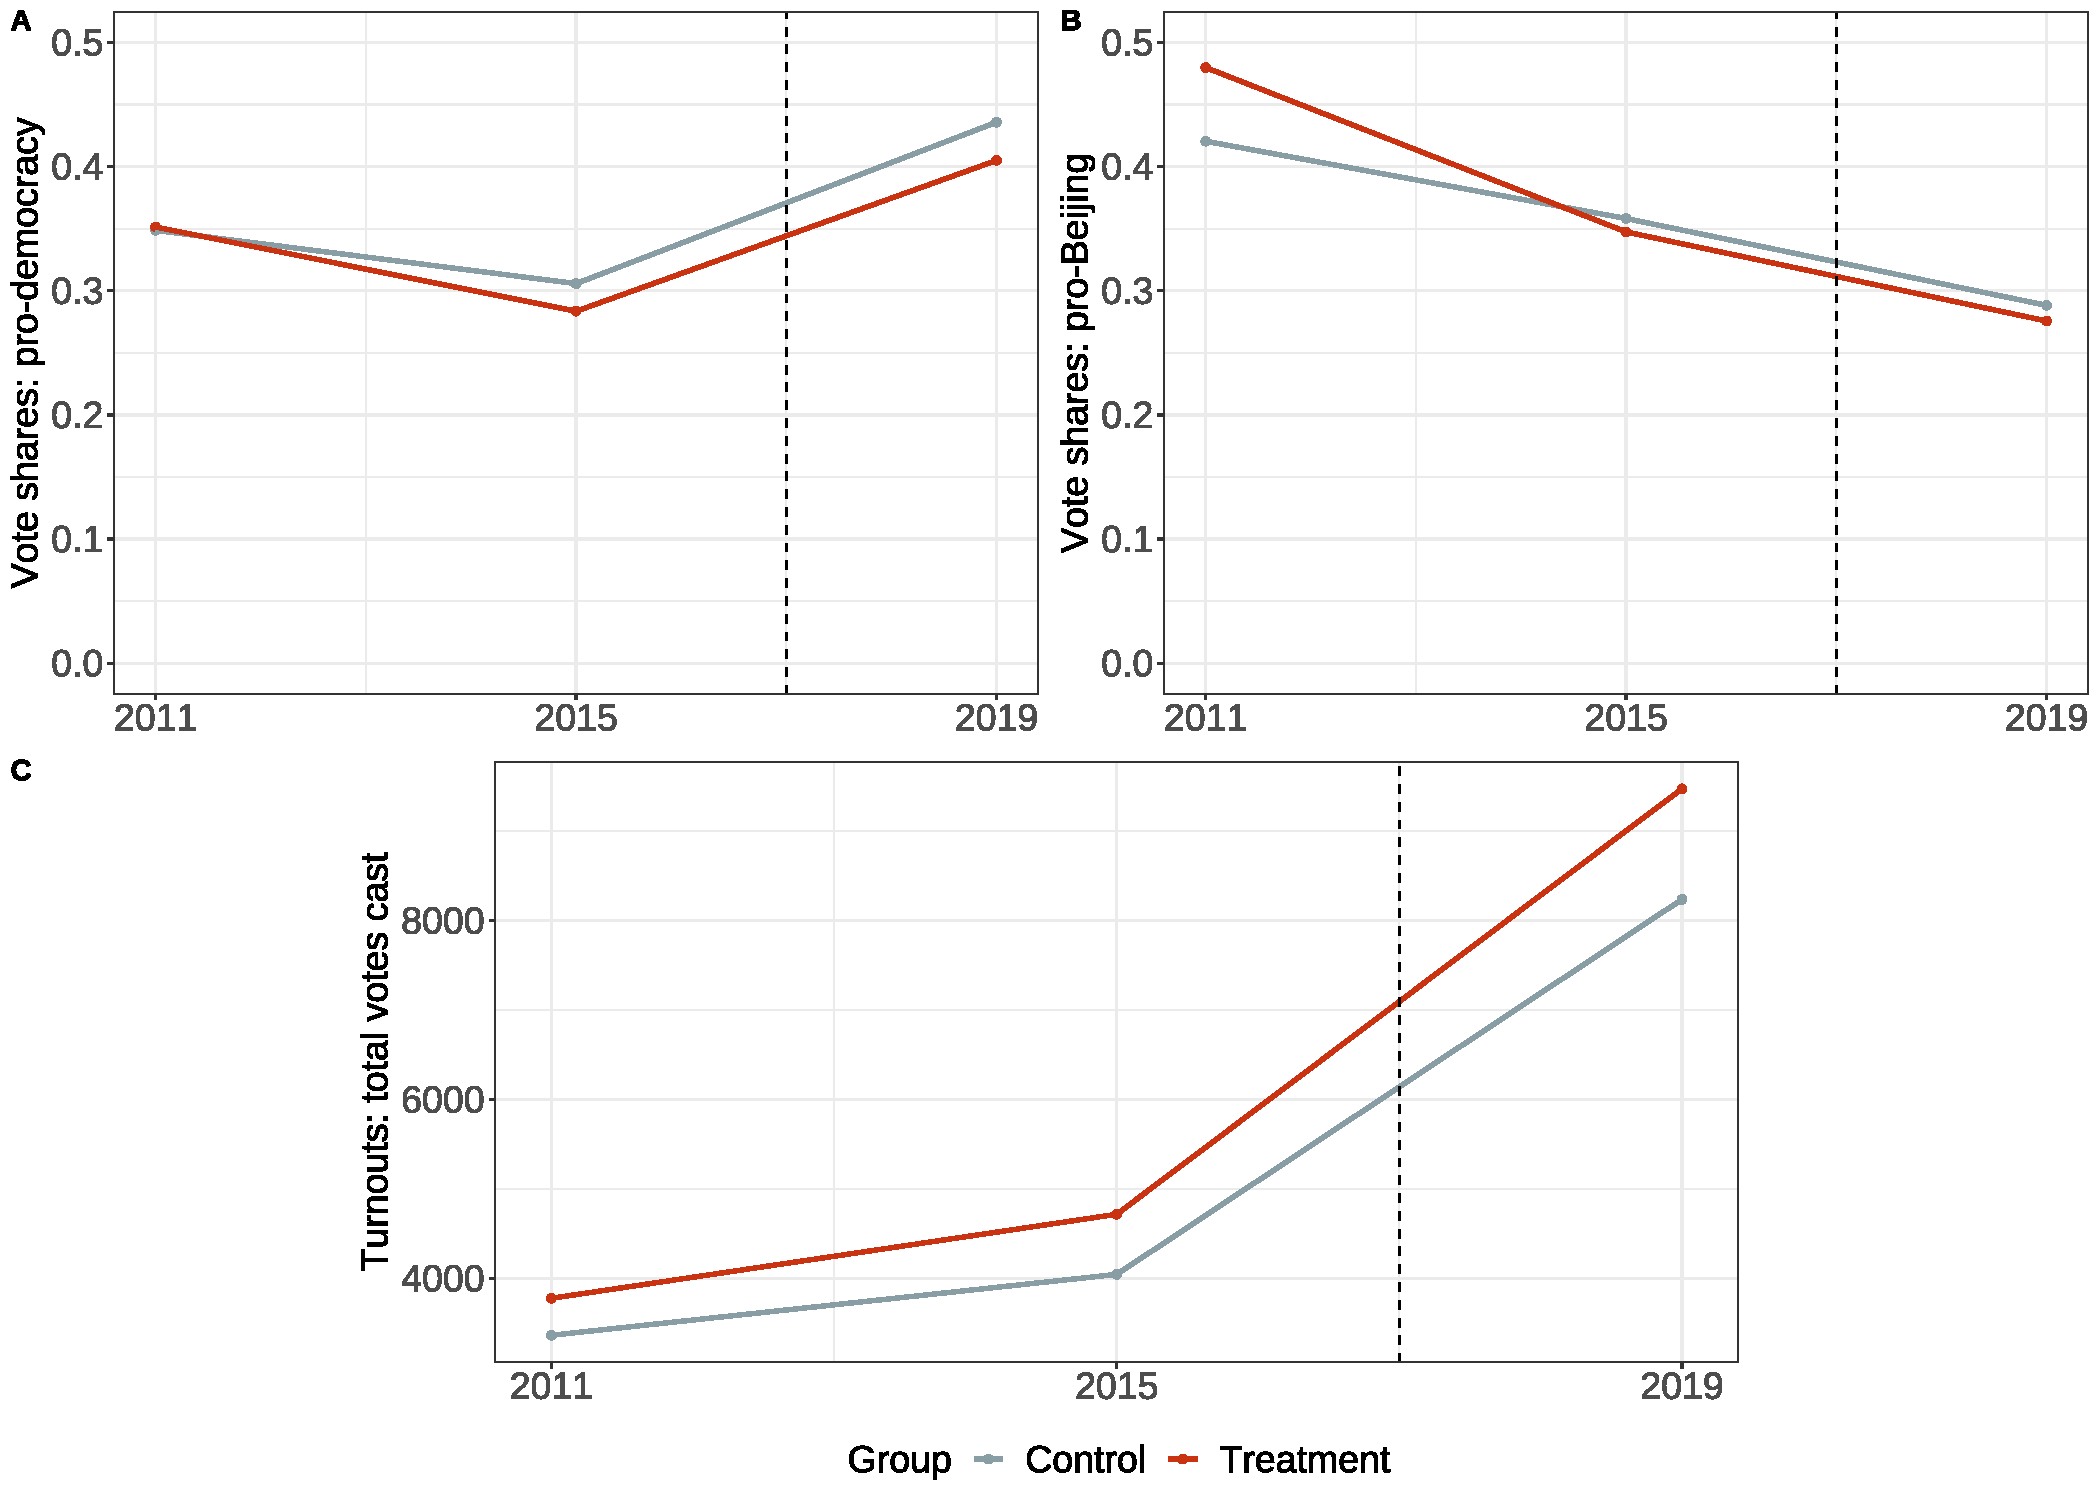
\includegraphics[width=16cm, height=12cm]{Visuals/parallel-trends-1.pdf}
    \caption{Vote share and turnout trends across the  control and treatment groups, 2011-2019.}
    \label{fig:paraltrends}
\end{figure}

Before I implement the difference-in-differences model, it is essential to verify whether the parallel trends assumption has been met. The parallel trend assumption is critical for a DiD analysis. It requires that during periods without the treatment, the outcomes for both the treatment group and the control group follow a similar trend  (Angrist and Pischke 2009; Cunningham 2021). Specifically in this case, the parallel trends assumption requires that the difference in each of the three election outcomes\footnote{The three outcomes are turnouts, vote shares for pro-democracy candidates, and vote shares for pro-Beijing candidates in a joined district} between the treated joined districts and the control joined districts remains constant before 2019 (Angrist and Pischke 2009; Cunningham 2021). As the Yellow Economic Circle was officially formed in 2019, this marks when the treatment of political consumerism was applied. 

Figure \ref{fig:paraltrends} shows the trends in both the treatment and control groups for all three outcomes. I define the treatment group as including joined districts with proportions of ``Yellow'' restaurants that are equal to or larger than the median proportion of the analysis data frame ($\approx 0.36$). Districts that do not meet this condition are categorized as the control group. The trends of both groups for the three outcomes remain largely parallel across the election years before the treatment in 2019 (Figure \ref{fig:paraltrends}). What is noteworthy, however, is that the trends also remain roughly parallel after the treatment (Figure \ref{fig:paraltrends}). Whether the electoral impact of the Yellow Economic Circle actually exists is further investigated in the next section.





\subsubsection{Difference-in-Differences with Two-Way Fixed Effects}

After verifying the parallel trends assumption, I implement difference-in-differences models with two-way fixed effects of the following forms for each of the three outcomes,
\begin{equation}
   Y_{it} = \gamma_{i} + \lambda_{t} + \delta YEC_i * Post_t + \epsilon_{it}, 
\end{equation}
\begin{equation}
    Y_{it} = \gamma_{i} + \lambda_{t} + \delta Majority_i * Post_t + \epsilon_{it},
\end{equation}
where $Y$ is the outcome of interest in a joined district $i$ of the year $t$. $YEC_{i}$, the treatment variable, is the proportion of ``Yellow'' restaurants in a joined district. $Majority_i$ is the binary indicator of whether the majority of politicized restaurants are ``Yellow'' in a joined district. Given that the treatment of the Yellow Economic Circle was applied in 2019, $Post_t$, the dummy variable, takes ``$0$'' before 2019 and ``$1$'' after. $\gamma_{i}$ denotes district fixed effects, and $\lambda_{t}$ denotes year fixed effects. The district fixed effects control for all time-invariant characteristics such as the projected population. The year fixed effects control for factors that affect all joined districts in both the treatment and the control groups in the same year, such as economic conditions in Hong Kong.





\clearpage
\section{Results}


% main tab---------------------------------------------------
\begin{table}[!h]
\centering\begingroup\fontsize{11}{12}\selectfont
\begin{tabular}{lcccccc}
\toprule
\multicolumn{1}{c}{ } & \multicolumn{2}{c}{\thead{Vote shares:\\pro-democracy}} & \multicolumn{2}{c}{\thead{Vote shares:\\pro-Beijing}} & \multicolumn{2}{c}{\thead{Turnouts:\\total votes cast}} \\
\cmidrule(l{3pt}r{3pt}){2-3} \cmidrule(l{3pt}r{3pt}){4-5} \cmidrule(l{3pt}r{3pt}){6-7}
 & (1) & (2) & (3) & (4) & (5) & (6)\\
\midrule
Proportion of ``Yellow'' restaurants & -0.065 &  & 0.031 &  & -239.395 & \\
\phantom{} & (0.059) &  & (0.043) &  & (831.241) & \\
Majority of restaurants are ``Yellow'' &  & -0.007 &  & 0.021 &  & -176.174\\
\phantom{} &  & (0.038) &  & (0.028) &  & (615.297)\\
\midrule
No. of obs. & 652 & 652 & 652 & 652 & 732 & 732\\
$R^2$ & 0.59 & 0.59 & 0.66 & 0.66 & 0.81 & 0.81\\
Year FE & Y & Y & Y & Y & Y & Y\\
District FE & Y & Y & Y & Y & Y & Y\\
\bottomrule
\multicolumn{7}{l}{\rule{0pt}{1em}*$p$ < 0.1; **$p$ < 0.05; ***$p$ < 0.01}\\
\end{tabular}
\caption{Main results: Difference-in-differences with TWFE.}
\label{tab:main_results}
\vspace{6pt}
\endgroup{}
{\fontsize{10}{11}\selectfont \raggedright \textbf{Notes}: Standard errors are clustered at the joined district level. ``Yellow'' restaurants are pro-democracy restaurants. \par}
\end{table}
% main tab---------------------------------------------------


\subsection{Main Results} \label{text:section5.1}
Table \ref{tab:main_results} presents the results from the main difference-in-differences analysis. For each of the three outcomes, I run two models using each of the two treatment variables. Standard errors for each model are clustered at the joined district level. A shift from 0 to 1 in the proportion of ``Yellow'' restaurants is associated with a decline of about 239 votes cast in a joined district (Table \ref{tab:main_results}, Column 5). It also appears that a shift from 0 to 1 in the proportion of ``Yellow'' restaurants is associated with an estimated decline of 6.5 percentage points in vote shares for pro-democracy candidates in a joined district (Table \ref{tab:main_results}, Column 1). However, a unit shift in the proportion of ``Yellow'' restaurants increases the shares for pro-Beijing candidates by 3.1 percentage points (Table \ref{tab:main_results}, Column 3). While these results contradict my argument, I fail to reject the null hypotheses for each of the three election outcomes at the 95 percent significance level (Table \ref{tab:main_results}). 

While using the binary treatment variable, I also did not find statistically significant evidence to support any of my hypotheses about the effect of having the majority of restaurants being ``Yellow'' on the three election outcomes (Table \ref{tab:main_results}, Columns 2, 4, and 6). On average, the total votes cast in districts with a majority of ``Yellow'' restaurants are approximately 176 less than those cast in districts without a majority (Table \ref{tab:main_results}, Column 6). Furthermore, the magnitude of the estimate of having the majority of ``Yellow'' restaurants (compared to not having the majority) on vote shares for pro-democracy candidates in a joined district is about -0.7 percentage points (Table \ref{tab:main_results}, Column 2), while that on vote shares for pro-Beijing candidates is 2.1 percentage points (Table \ref{tab:main_results}, Column 4). But again, those results are statistically insignificant.

Overall, I did not find any measurable effect of the YEC on all three outcomes, regardless of whether I used a continuous or binary treatment variable. 




\paragraph*{Heterogeneous Treatment Effects } 
In addition, I consider two dimensions of heterogeneity in my analysis. I divide the joined districts into two subgroups to see if the effect of the proportion of ``Yellow'' restaurants on vote shares for pro-democracy candidates varies across different groups. 

\vspace{6pt}
%\paragraph*{Heterogenity Effects}
\begin{figure}[!h]
    \centering
    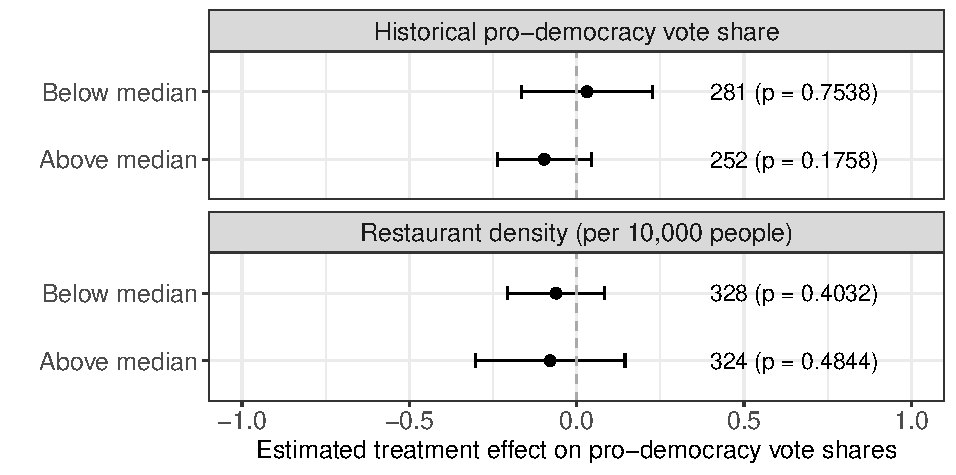
\includegraphics[width=13cm, height=6.5cm]{Visuals/hte.pdf}
    \caption{Subgroup effects on vote shares for pro-democracy candidates in a joined district.}
    \floatfoot{\textbf{Notes}: Standard errors are clustered at the joined district level. Horizontal lines show the 95\% confidence intervals for each estimate. The number of observations for each subgroup and the $p$-value for each estimate are annotated on the right side of the plot.}
    \label{fig:hte}
\end{figure}

For the first dimension, I divide the joined districts by the median historical vote shares for pro-democracy candidates. To measure historical vote shares, I calculate the mean pro-democracy vote shares in a given District Council Constituency (DCC) for both 2011 and 2015. Then after joining the DCCS, I separate joined districts into two groups based on whether their historical pro-democracy vote share is above the median or not. 

The second dimension considers whether the politicized restaurant density is below or above the median density affects my conclusion. To compute the restaurant density, I divide the number of politicized restaurants by the projected population\footnote{Data for the projected population of each original DCC in an election year are also available on the Government of HKSAR's websites. See Appendix \ref{appendix:election_data}.} in ten-thousands of a joined district in 2019. 

Based on Figure \ref{fig:hte}, which visualizes the estimated treatment effect on both subgroups, I find no statistically significant treatment effect for the two smaller groups within two larger subgroups.  








\subsection{Protests as An Alternative Mechanism}
\begin{figure}[!h]
    \centering
    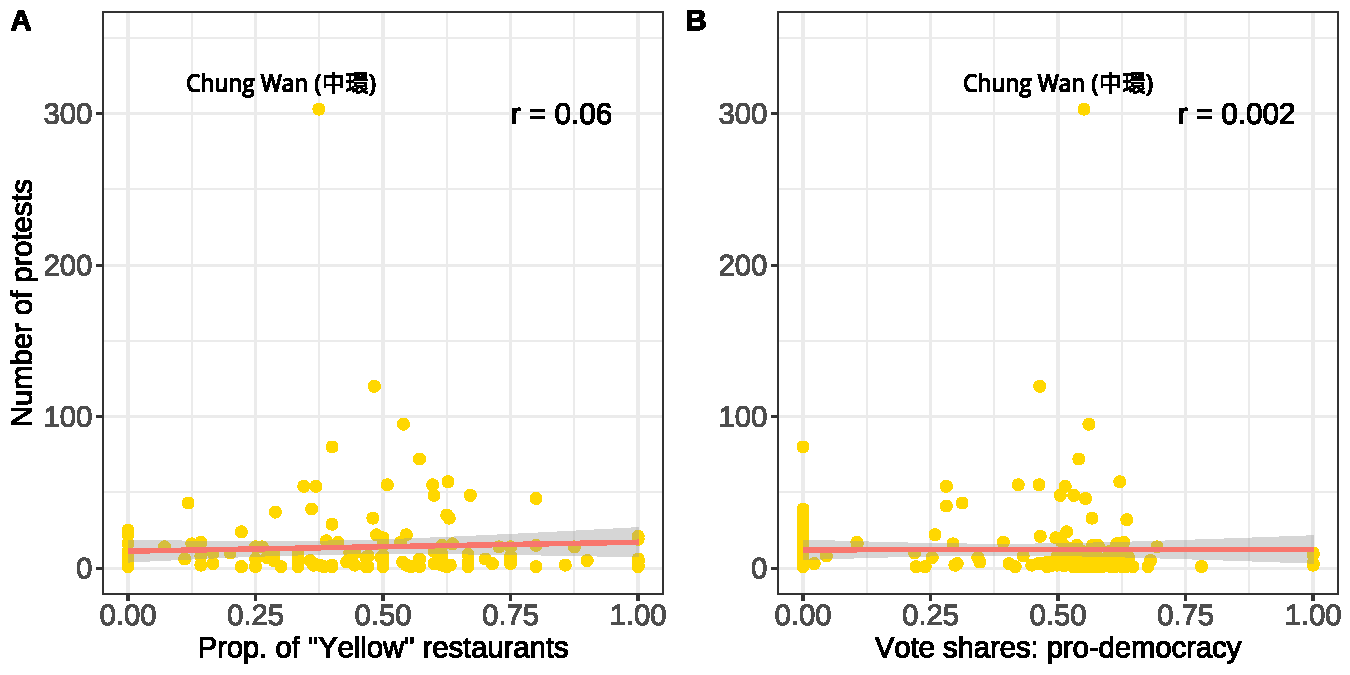
\includegraphics[scale=0.7]{Visuals/plt_cor_protests.pdf}
    \floatfoot{\textbf{Notes}: Shaded areas are the 95\% confidence intervals. There is an outlier, Chung Wan (covering a significant portion of Central, the political and business center), in both scatter plots. If this data point is excluded, the correlation is 0.11 for Figure 9.A and -0.04 for Figure 9.B.}
    \caption{Correlations with the number of protests in a joined district. (Source: HKU)}
    \label{fig: cor_protests}
\end{figure}

Given that mass protests took place concurrently with the formation of the YEC in 2019, I also investigate an alternative mechanism described in the theory section (Section \ref{section:alternative_mechanism}). Protests in 2019 were organized in city centers where restaurants are often clustered. Is it possible that the ``Yellow'' restaurants promoted more protests in a joined district? Researchers at the University of Hong Kong (HKU) recorded both temporal and spatial data for pro-democracy protests\footnote{See \url{https://antielabdata.jmsc.hku.hk/} for more details.}. Using those data, I conduct a correlation analysis to see if larger proportions of ``Yellow'' restaurants are associated with higher frequencies of protests in a joined district in 2019. I also investigate the correlation between the number of protests and the vote shares for pro-democracy candidates in a joined district in 2019. Those relationships are shown in scatterplots in Figure \ref{fig: cor_protests}. While positive, both correlations are extremely weak: The correlation between the proportion of ``Yellow'' restaurants and the frequency of protests is $0.06$, while the correlation between the proportion of ``Yellow'' restaurants and the vote shares for pro-democracy candidates is $0.002$ (Figure \ref{fig: cor_protests}).

However, it is noticeable that there is an outlier, Chung Wan (\begin{CJK*}{UTF8}{bkai}中環\end{CJK*}), in both Figures \ref{fig: cor_protests}A and \ref{fig: cor_protests}B. This outlier alone recorded 330 protests in 2019. Covering most areas of the Central District\footnote{See Figure \ref{fig: heatmap} for a rough indication of its location.}, this DCC is the financial and political center of Hong Kong. Most protests in 2019---or any other previous anti-authoritarian movements in Hong Kong---had therefore chosen this DCC as their focal point. The protesters' goal was to effectively coordinate collective actions. When this outlier is removed, the correlations for both relationships change to $0.11$ and $-0.04$, respectively (Figure \ref{fig: cor_protests}). Those correlations are still close to negligible when the outlier is removed. 

Undoubtedly, a correlation analysis that only takes data for the year 2019 into account is less methodologically rigorous than the difference-in-differences model that fits panel data in my main results. However, it adds additional support to the conclusion from the main results: The YEC might not have encouraged more protests, and there has also been an extremely weak association between the number of protests and vote shares for pro-democracy candidates in a joined district in 2019. 





\subsection{Robustness Checks}

\begin{table}[!h]
\centering\begingroup\fontsize{10}{11}\selectfont
\caption{Results with different numbers of joined districts excluded.}
\vspace{6pt}

\begin{tabular}{lccc}
\toprule
\multicolumn{1}{c}{ } & \multicolumn{1}{c}{\thead{Vote shares:\\pro-democracy}} & \multicolumn{1}{c}{\thead{Vote shares:\\pro-Beijing}} & \multicolumn{1}{c}{\thead{Turnouts:\\total votes cast}} \\
\cmidrule(l{3pt}r{3pt}){2-2} \cmidrule(l{3pt}r{3pt}){3-3} \cmidrule(l{3pt}r{3pt}){4-4}
 & (1) & (2) & (3)\\
\midrule
\textbf{Panel A: All joined districts excluded} & \phantom{} & \phantom{} & \phantom{}\\

Proportion of ``Yellow'' restaurants & -0.065 & 0.032 & -383.699\\
 & (0.067) & (0.050) & (344.704)\\
No. of obs. & 500 & 500 & 579\\
$R^2$ & 0.59 & 0.66 & 0.81\\
\midrule
\textbf{Panel B: Joined DCCs $\geq$ 4 excluded} & \phantom{} & \phantom{} & \phantom{}\\

Proportion of ``Yellow'' restaurants & -0.069 & 0.032 & 142.487\\
 & (0.061) & (0.045) & (518.837)\\
No. of obs. & 589 & 589 & 669\\
$R^2$ & 0.59 & 0.66 & 0.83\\
\midrule
\textbf{Panel C: Joined DCCs $\geq$ 5 excluded} & \phantom{} & \phantom{} & \phantom{}\\

Proportion of ``Yellow'' restaurants & -0.077 & 0.036 & 45.346\\
 & (0.060) & (0.044) & (563.773)\\
No. of obs. & 610 & 610 & 690\\
$R^2$ & 0.59 & 0.66 & 0.84\\
\midrule
\textbf{Panel D: Joined DCCs $\geq$ 6 excluded} & \phantom{} & \phantom{} & \phantom{}\\

Proportion of ``Yellow'' restaurants & -0.068 & 0.030 & -337.141\\
 & (0.059) & (0.044) & (598.212)\\
No. of obs. & 622 & 622 & 702\\
$R^2$ & 0.60 & 0.66 & 0.84\\
\midrule
Year FE & Y & Y & Y\\
District FE & Y & Y & Y\\
\bottomrule
\multicolumn{4}{l}{\rule{0pt}{1em}*$p$ < 0.1; **$p$ < 0.05; ***$p$ < 0.01}\\
\end{tabular}
\label{rc:joined_districts}
\endgroup{}
\floatfoot{\RaggedRight \textbf{Notes}: Standard errors are clustered at the joined district level.}
\end{table}


I run three robustness checks on my main DiD models in Section \ref{text:section5.1} to verify if my conclusion remains robust to several factors that might affect my results. I begin by assessing if large joined districts resulting from my method to create panel data will affect my conclusion. Then I test if those uncontested DCCs where candidates were automatically elected will change my conclusion. Lastly, I also test if using different assumptions when I finalize data for the politicized restaurant set will result in different conclusions. Overall, my conclusion from the main analysis is reliable and valid even when I take those factors into account.

\paragraph*{Large Joined Districts}
The first robustness check serves to test if the null results from my main conclusion are robust to including different numbers of those joined districts I manually created. There is a trade-off between observing more geographically consistent units and losing some variation in votes cast at a more granular level due to combining several districts that had been drastically redistricted. I generate four additional panels with different numbers of joined districts removed to see if my conclusion still holds when large joined districts are not included. For example, Panel B excludes joined districts with the number of raw District Council Constituencies (DCC) larger or equal to four (Table \ref{rc:joined_districts}). 

Table \ref{rc:joined_districts} presents the DiD estimates when panels with different numbers of excluded joined districts are used. I find no statistically significant evidence that the proportion of ``Yellow'' restaurants in a joined district increases turnouts and vote shares for pro-democracy candidates when different numbers of large joined districts are used (Table \ref{rc:joined_districts}, Columns 1 and 3). There is also no statistically significant finding for whether the proportion of ``Yellow'' restaurants increases vote shares for pro-Beijing candidates as well (Table \ref{rc:joined_districts}, Column 2). This supports that my conclusion from the main analysis is robust to large joined districts.


\vspace{9pt}
\begin{table}[!h]
    \centering \fontsize{10}{11}\selectfont
    \caption{Number of candidates in uncontested DCCs by political ideology ($n = 144$).}
    \vspace{6pt}
    \begin{tabular}{||c|c|c||}
     \hline
     \textbf{Pro-Democracy}   &  \textbf{Pro-Beijing} & \textbf{Independent}\\
     \hline \hline
      3 (2\%)   & 92 (64\%) & 49 (34\%)\\
     \hline
    \end{tabular}
    \label{tab:uncontested_by_ideo}
\end{table}
\begin{table}[!h]
\centering\begingroup\fontsize{10}{12}\selectfont
  \caption{Results with uncontested DCCs.}
  \label{tab: results_uncontested}
\vspace{3pt}
\begin{tabular}{lcc}
\toprule
\multicolumn{1}{c}{ } & \multicolumn{1}{c}{\thead{Vote shares:\\pro-democracy}} & \multicolumn{1}{c}{\thead{Vote shares:\\pro-Beijing}} \\
\cmidrule(l{3pt}r{3pt}){2-2} \cmidrule(l{3pt}r{3pt}){3-3}
 & (1) & (2)\\
\midrule
\textbf{Panel A: All joined districts excluded} & \phantom{} & \phantom{}\\
Proportion of ``Yellow'' restaurants & -0.015 & -0.008\\
 & (0.067) & (0.051)\\
No. of obs. & 578 & 578\\
\midrule
\textbf{Panel B: Votes cast in joined districts interpolated} & \phantom{} & \phantom{}\\
Proportion of ``Yellow'' restaurants & -0.029 & 0.001\\
 & (0.059) & (0.045)\\
No. of obs. & 731 & 731\\
\midrule
$R^2$ & 0.58 & 0.64\\
Year FE & Y & Y\\
District FE & Y & Y\\
\bottomrule
\multicolumn{3}{l}{\rule{0pt}{1em}*$p<0.1$; **$p<0.05$; ***$p<0.01$}\\
\end{tabular}
\endgroup{}
\floatfoot{\RaggedRight \textbf{Notes}: Standard errors are clustered at the joined district level.}
\end{table}

\paragraph*{Uncontested Districts}
In the finalized analysis data frame I use to fit my main models, I exclude those uncontested DCCs where there was only one candidate running. Those uncontested DCCs only presented in the 2011 and 2015 elections. The raw votes cast for those candidates are missing as they were automatically elected. To test the impact of those uncontested districts on my analysis, I try to fill in the missing data and run the DiD analysis again. I retrieve their declared political affiliations from the Government of HKSAR's websites and categorize those candidates into each political ideological group. As Table \ref{tab:uncontested_by_ideo} shows, pro-Beijing candidates accounted for around 64\% of those elected to uncontested DCCs in 2011 and 2015. Pro-democracy candidates constituted only 2\% of this group. 

For candidates who ran for an uncontested DCC that remained 90\% unchanged across the three election years, I manually set the vote share for their given political ideological group in proportion to one. However, it is challenging to fill in the vote shares for candidates running in DCCs that require me to create a joined district. This is again because there was no information about the number of votes cast for a candidate in an uncontested DCC. While I fully acknowledge that this may not be a methodologically perfect solution, I interpolate raw votes cast based on that candidate's political affiliation in that uncontested DCC using a linear method and votes cast for the other two years recorded. If votes are also missing for two other election years for a candidate in a DCC, I interpolate the number by considering votes cast for other contiguous DCCs in that specific year (the two DCCs belong in the same joined district; most of the time one was split from another). Then I sum the votes for different political ideological groups at the joined district level and calculate the shares for each group. 


Doing so allows me to test whether those uncontested candidates will affect my calculations for vote shares based on political ideologies and my conclusion as a whole. I generate another two panels: Panel A excludes all those interpolated data by removing observations for all joined districts, while Panel B includes them. Results from those panels show that larger proportions of ``Yellow'' restaurants in a joined district are associated with a decline in vote shares for pro-Beijing candidates: 1.5 percentage points if I use Panel A, and 2.9 percentage points if I use Panel B with interpolated data (Table \ref{tab: results_uncontested}, Column 1). But again, those results are not significant at the 95\% level. Therefore, this check adds additional support to my conclusion: The main results still remain robust without uncontested districts (Table \ref{tab: results_uncontested}).




\paragraph*{Closed restaurants}
%\clearpage
\begin{table}[!h]
    \centering \fontsize{10}{11}\selectfont
    \caption{Number of closed restaurants by political ideology ($n = 1162$).}
    \vspace{3pt}
    \begin{tabular}{||c|c||}
     \hline
     \textbf{Yellow}   &  \textbf{Blue}\\
     \hline \hline
      491 (42\%)   & 671 (58\%)\\
     \hline
    \end{tabular}
    \label{tab:closed_set}
\end{table}



%\clearpage
\begin{table}[!h]
\centering\begingroup\fontsize{10}{12}\selectfont
  \caption{Results with closed restaurants (No.\ of politicized restaurants = 3874).}
\vspace{6pt}

\begin{tabular}{lcccccc}
\toprule
\multicolumn{1}{c}{ } & \multicolumn{2}{c}{\thead{Vote shares:\\pro-democracy}} & \multicolumn{2}{c}{\thead{Vote shares:\\pro-Beijing}} & \multicolumn{2}{c}{\thead{Turnouts:\\total votes cast}} \\
\cmidrule(l{3pt}r{3pt}){2-3} \cmidrule(l{3pt}r{3pt}){4-5} \cmidrule(l{3pt}r{3pt}){6-7}
 & (1) & (2) & (3) & (4) & (5) & (6)\\
\midrule
Proportion of ``Yellow'' restaurants & -0.034 &  & 0.006 &  & -69.051 & \\
\phantom{} & (0.061) &  & (0.044) &  & (862.359) & \\
Majority of restaurants are ``Yellow'' &  & 0.011 &  & 0.022 &  & 176.499\\
\phantom{} &  & (0.036) &  & (0.027) &  & (643.007)\\
\midrule
No. of obs. & 692 & 692 & 692 & 692 & 777 & 777\\
$R^2$ & 0.60 & 0.60 & 0.66 & 0.66 & 0.80 & 0.80\\
Year FE & Y & Y & Y & Y & Y & Y\\
District FE & Y & Y & Y & Y & Y & Y\\
\bottomrule
\multicolumn{7}{l}{\rule{0pt}{1em}*$p$ < 0.1; **$p$ < 0.05; ***$p$ < 0.01}\\
\end{tabular}
\label{tab:results_closed}
\endgroup{}
\floatfoot{\RaggedRight \textbf{Notes}: Standard errors are clustered at the joined district level.}
\end{table}

The third robustness check aims to assess if keeping those ``Closed'' restaurants in my analysis data frame will produce different conclusions for the findings about the three outcomes. When constructing the analysis data frame for the main models, I exclude those restaurants added before the 2019 election but indexed as ``Closed'' on OpenRice, the food service review platform. I do so because I cannot obtain information about when exactly a restaurant has been permanently closed. It is very possible that a good number of them might have not shut down before the 2019 election and therefore be capable of shaping voting behavior. Therefore, I run another robustness check using a different analysis data frame in which 1,162 closed (but indexed as added before the election) politicized restaurants were included (see Table \ref{tab:closed_set} for tabulated statistics of this closed set). Mapping a total of 3,874 restaurants to their respective joined districts, I recalculate the proportion of ``Yellow'' restaurants and create another binary indicator with the same cutoff rule ($Pr_{yellow} \geq 0.5$). Then I fit another 6 DiD models with two-way fixed effects in the same form as that in the main analysis. My conclusion from the main results still remains robust after I perform the test: I find no statistically significant evidence that the YEC increases turnouts and vote shares for pro-democracy candidates if those restaurants whose operational statuses I cannot verify are added (Table \ref{tab:results_closed}).

The three robustness checks produce results that are consistent with the null finding from my main results in Section \ref{text:section5.1}: I do not find sufficient statistical evidence that the proportion of ``Yellow'' restaurants in a joined district affects turnouts and vote shares for both pro-democracy and pro-Beijing candidates.




\section{Concluding Remarks}

\subsection{Discussion}

Robert A.\ Dahl (1971, 15) famously stated that ``the more the cost of suppression exceeds the costs of toleration, the greater the chance for a competitive regime.'' When reviewing prior literature on anti-authoritarian movements and conceptualizing the case of Hong Kong, I argue that the cost of suppressing political consumerism campaigns for an authoritarian government is high as it requires an enormous amount of effort to suppress individual consumption decisions. This is, again, because citizens are able to conceal their support by framing it as quotidian decisions on choosing a place to eat. In the meantime, they can infer fellow consumers' political preferences, learn more about pro-democracy candidates in this low-salience election, and reveal their true preferences at the polling stations (Kuran 1991). If these mechanisms were true, pro-democracy businesses and citizens might be able to resist democratic backsliding by reinforcing their democratic political ideologies, encouraging more people to vote, and electing pro-democracy candidates (Lindberg 2009).

The statistically insignificant results from my analysis indicate that those political consumerism campaigns, even though broad-based, may not have the proposed downstream effects on voter turnouts and election outcomes. This might sound frustrating to both pro-democracy businesses and citizens who aim to use the institutional strategy to resist democratic erosion (Gamboa 2017; Lindberg 2009). However, this null finding does not imply that mass political consumerism campaigns of the Yellow Economic Circle do not produce any political impact at all.

I speculate several reasons for these null results and why overall the Yellow Economic Circle was a weak treatment. A very simple explanation is that people may not take politics into consideration when making their food choices. Sometimes customers may prioritize food quality and locations. For example, a restaurant that consistently offers exceptionally good food may be able to attract and retain customers who will ignore the owner's political beliefs. Moreover, working overtime has been a culture in Hong Kong. Sometimes when people leave work and become hungry at late hours, they may not have instant access to substitutes even though they know that the restaurant owners may oppose their political support. 
    
What is also worth discussing is that customers might have already known the political preferences of many restaurant owners long before the YEC's formation and the election. A large proportion of Hong Kong's food service industry has been comprised of community-based businesses (\begin{CJK*}{UTF8}{bkai}``街坊生意''\end{CJK*}). Many customers regularly dine at this type of restaurant and have become acquainted with the owners. Again, due to the limited living environment, it is easy for Hong Kong citizens to infer people's political support in a community before an election (Stokes 2015). In this case, the YEC may not generate an effective electoral impact by reinforcing and promoting existing pro-democracy ideals to sway voters.


Furthermore, many people may not be interested in a low-salience local election. The District Council Election is seen as relatively less high-stakes as compared to the Legislative Council Election and the Chief Executive Election in Hong Kong. Even if candidates declare political affiliations with certain political parties, their policy proposals might have still focused on low-level issues within the community, which might be seen as trivial to voters. Even though the YEC raises awareness for this 2019 election by providing information about the pro-democracy ideals, it is possible that some voters might have formed a belief that voting for pro-democracy candidates running for a low-salience election would not generate far-reaching political impact, thereby refraining from voting specifically for pro-democracy candidates, regardless whether they have been exposed to the YEC or not.


Another rationalization for the weak treatment of the Yellow Economic Circle is that many people who do not live in an electoral democracy may not be interested in formal politics such as elections overall. Previous research suggests that as compared to citizens residing in liberal democracies, citizens in electoral autocracies, or a hybrid regime like Hong Kong, may not feel a strong civic duty to vote in elections (Letsa 2020; Reuter 2021). Some believe that such elections are frauds, while some may choose to abstain from voting to show their opposition to the political regime (Frantz 2018; Magaloni 2006; Letsa 2020; Reuter 2021).


Methodologically, the year and district fixed effects I threw in my difference-in-differences models may not perfectly capture all time-varying variables. For example, the model may not capture the effect of population sorting over the years. There has been a surge of emigration among Hong Kong citizens since 2014 after the Umbrella Movement. Lim (2023) presents empirical evidence that emigration affects voting behavior in the home-sending countries. 

In addition, the disqualifications and incarceration of pro-democracy candidates and incumbents over the years, in particular during the 2019 Anti-ELAB Movement. Joshua Wong Chi-Fung, a prominent figure in Hong Kong's anti-authoritarian movements since 2014, was disqualified from running for the 2019 District Council Election by the government. Nathan Law Kwun-Chung, another outspoken and preeminent pro-democracy activist and former politician, sought asylum in the U.K. If no pro-democracy candidate is running in a joined district, or if those Hong Kong citizens who are supposedly more likely to vote for pro-democracy candidates have already left, the vote shares for partisan candidates can be impacted (Lim 2023).


\subsection{Limitations}
There are some limitations of this thesis, especially in terms of the data I am using. One limitation lies in the politicized restaurant data. Because I rely on crowdsourced data from a social media review platform, certain biases exist. Notably, negativity bias may affect the number of ``Blue'' restaurants reported by pro-democracy users. Negative bias describes the situation in which people are more inclined to be stimulated by negative information around them (Vaish et al.\ 2008). It is possible that ``Blue'' restaurants are therefore overrepresented in my data set. That being said, pro-democracy users may have paid more attention to identifying and reporting restaurants or restaurant owners whose ideology is not in alignment with theirs. Moreover, some restaurant owners may also falsify their political support when they see the prospect of economic benefits encompassed by the momentum of the Yellow Economic Circle. OpenRice users have reported several instances of pro-establishment restaurant owners falsifying support for pro-democracy protests.


Although I have used what I believe to be the best practice available to ensure data quality (such as taking whether a store is part of a chain business into account and consulting other crowdsourced platforms), it is challenging to acquire data that accurately represent those restaurants whose political preferences are correctly and timely identified during the formation of the YEC but not after the 2019 District Council Election. 

Another limitation of this thesis is that I relied on partisanship as an indicator of candidates' political ideologies. A small number of members of both the pro-democracy and pro-Beijing groups chose to run as independent candidates. Among them, Junius Ho Kwan-Yiu has been famous for his pro-Beijing advocacy and persistent denouncement of social movements in Hong Kong. If feasible, estimating a candidate's political preferences using roll-call votes would have better captured ideological preferences for individual independent candidates over the years and give a less arbitrary indicator of political ideologies (e.g. an algorithm proposed by Imai et al.\ (2016) to estimate ideal points). However, those data are not available in the case of Hong Kong's District Council Elections. While I have incorporated multiple sources to improve how I categorize candidates, partisanship alone may not capture the political dynamics among independent candidates.



\subsection{Future Research}
This thesis aims to bring the existing literature on political consumerism and democratic backsliding into conversation with one another. Whereas prior research largely focuses on established democracies, investigating the case of Hong Kong---a hybrid regime---adds nuances to our understanding of the electoral impact of political consumerism campaigns. Furthermore, this thesis tests a newly emerging research question in democratic backsliding: whether social movements led mostly by private businesses and citizens alone can provide effective resistance to elite-led democratic erosion. While I did not find statistically significant evidence for effective resistance, the data collected for such a large number of politically expressive restaurants demonstrate that private businesses, typically seen as being motivated solely by economic profits, can also be ideologically sincere once in a while. 

Future research can benefit from looking into additional cases of broad-based political consumerism campaigns at an individual level. Different methods can be used to amend the possible decoupling between the identities of voters and politically aware consumers. Some research designs, such as surveys, may be able to reduce the impact of some factors that affect voters/politically aware consumers' decision-making process, such as the convenience of restaurant locations (i.e.\ Some people may not necessarily choose to eat in their registered constituency when they leave work.). 

A well-designed field experiment, if feasible, may be able to compensate for the inherent deficiencies of quasi-experimental designs like the one presented in this thesis. For example, there could be a field experiment before a U.S. election where randomly selected stores are asked to put up signs to indicate their support for a candidate. Customers are asked about which candidates they are most likely to vote for after seeing the signs before the election and whom they actually vote for after. Turnouts in the specific community where those politicized restaurants are located can be compared with those that do not show a sign. Whether there could be spillover effects on other types of businesses following the practice of those politicized restaurants can also be estimated. 

Is ``gastropopulism'' a solid concept? While empirical evidence presented in this thesis is from a single case study of a hybrid regime, it still has implications for countries experiencing democratic erosion elsewhere and contributes to our understanding of how future research can proceed. 



%------------------------------References
\pagebreak
\begingroup
\setstretch{1.5}
\setlength\bibitemsep{6pt}
\printbibliography[heading=bibintoc]
\endgroup


%----------------------------------------------------------------
%-------------------------Appendices-----------------------------
%----------------------------------------------------------------
\pagebreak
\begin{appendices}
\setstretch{1.5}

\section{Restaurant Categorization System} \label{appendix:categorization_system}

\subsection{Examples: OpenRice User Comments} \label{appendix:openrice_usercomments}
The list below displays selected comments left by pro-democracy OpenRice users to help the crowdsourced account better categorize restaurants. I translated those comments originally in Cantonese to English. They describe users' personal dining experiences and observations about restaurant owners' political stances amid the protests.

\begin{itemize}
    \small
    \item \textbf{Yellow}: \begin{CJK*}{UTF8}{bkai}``616火鍋係黃的, 叫人登記做選民 ~\& 8月5有罷工。''\end{CJK*} [616 Hot Pot is a Yellow restaurant. They reminded people to register to vote and went on strike on August 5th (referring to the city-wide strike on August 5th organized by pro-democracy protesters).]
    
    \item \textbf{Yellow}: \begin{CJK*}{UTF8}{bkai}``籽樂廚房是黃的。10.2表示黃藍是政見,黑白是良知!\#香港人加油!11.11罷工但開放餐廳提供免費食物俾有需要既人,當日收到既全部錢都捐到星火同立場。''\end{CJK*} [Sowergift Kitchen is a Yellow restaurant. They stated (on their official website) on October 2nd that ``Yellow'' and ``Blue'' are different political stances, but [what is going on in the city] is actually about conscience. \# Fight, Hong Kongers! They went on strike on November 11st, but their restaurant remained open and offered free food to pro-democracy protesters in need. They said they would donate all of their revenues on that day to Spark Alliance (a citizen-led group that offers legal assistance to arrested protesters) and Stand News (a local pro-democracy news platform).]
    
    \item \textbf{Blue}: \begin{CJK*}{UTF8}{bkai}``紅磡中華小廚, 收銀阿姐(老細)唔止一次鬧示威者攪亂哂個社會, 阻左哂人搵食。本身隔日食早餐, 而家不了。''\end{CJK*} [At the Mid-Dynasty Restaurant in Hung Hom, the cashier (also the owner of the restaurant) repeatedly said that (pro-democracy) protesters disrupted the society, preventing people from making a living. I used to go there for breakfast every other day, but not anymore.]
    
    \item \textbf{Blue}:
    \begin{CJK*}{UTF8}{bkai}``大家成日話罷食黑建幫嘅富臨,但係我好驚訝你哋竟然忽略咗8月5同9月15日有份喺明園西街衝出嚟打人嘅《大紅袍火鍋料理》老闆!老闆本身係福建頭目,多次揚言要打死曱甴,仲組織北角炮台山恐襲!最近佢仲同人合資開多間《樓下火鍋飯店》。我每次經過大紅袍都仲見到人頭湧湧,香港人,你哋知點做啦!!''\end{CJK*} [People are talking about boycotting the Fulum Group owned by the Fujiang gang, but I am surprised that you guys all neglect the owner of Da Hong Pao Hot Pot, who violently attacked pro-democracy protesters during the riots in Ming Yuen Western Street on August 5th and September 15th. The owner is an important member of the Fujiang gang, who repeatedly said they would beat the cockroaches (a slur for pro-democracy protesters) and organize attacks in North Point and Fortress Hill. The owner partnered with others to open many restaurants named Lau Haa Hot Pot. Every time I passed by, I saw so many people dine at Da Hong Pao. Fellow Hong Kongers, you know what to do!]
\end{itemize}

\subsection{Images of ``Yellow'' Restaurants} \label{appendix:yellow_sticker_slogan}

\begin{figure}[!h]
    \centering
    \subfloat[\centering The slogan at a ``Yellow'' cafe. (Source: @handstopmouthstop)]{{
\includegraphics[width=6cm, height=4cm]{Visuals/slogan-yellow.jpeg} }}%
    \qquad
    \subfloat[\centering The sticker at a ``Yellow'' restaurant. (Source: Radio Free Asia)]{{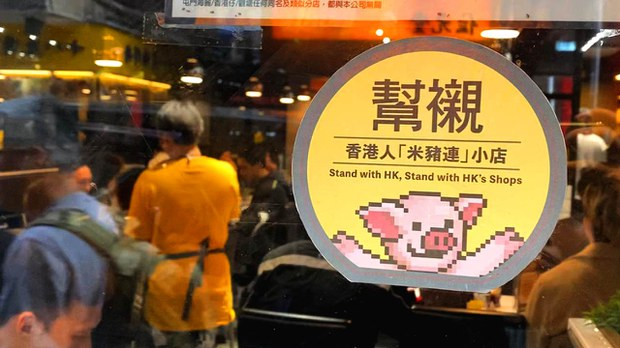
\includegraphics[width=6cm, height=4cm]{Visuals/yellow-stickers.jpeg} }}
    \label{fig:sidebyside}
\end{figure}
The most popular slogan during the Anti-ELAB Movement, ``Free Hong Kong, revolution of our time (\begin{CJK*}{UTF8}{bkai}``光復香港,時代革命''\end{CJK*}), is displayed in Figure A.2(a)\footnote{Source: \url{https://tinyurl.com/2mmxnl73}}. Figure A.2(b)\footnote{Source: \url{https://tinyurl.com/2dwngwdy}} shows an example of the sticker made by pro-democracy restaurant owners and consumers to signal their political preferences, which imitates the practice of the MICHELIN Guide (\begin{CJK*}{UTF8}{bkai}``米豬蓮''\end{CJK*} sounds like \begin{CJK*}{UTF8}{bkai}``米芝蓮''\end{CJK*}, the Cantonese translation of ``MICHELIN''). The largest two Traditional Chinese characters in Figure A.2(b), \begin{CJK*}{UTF8}{bkai}``幫襯''\end{CJK*}, represent ``deliberately support'' in both Cantonese and Mandarin. In this case, they also imply the concept of ``buycotts.'' 



\phantom{}\\
\phantom{}\\








\section{Election Data} \label{appendix:election_data}
% table
%\clearpage
\newcolumntype{C}{>{\RaggedRight\arraybackslash}X}
\begin{table}[h!]
\setlength\extrarowheight{2pt} % for a bit of visual "breathing space"
\begin{tabularx}{\textwidth}{CCCCCC}
\toprule
\textbf{Year} & \textbf{Type} & \textbf{Electoral Rule} & \textbf{No.\ of DCCs} & \textbf{No.\ of Polling Stations} &\textbf{Link}  \\
\midrule
\cellcolor{gray!6}{2019} &  \cellcolor{gray!6}{District Council Election}  & \cellcolor{gray!6}{First-past-the-post} & \cellcolor{gray!6}{452} & \cellcolor{gray!6}{605} & \cellcolor{gray!6}{\url{tinyurl.com/2mshxtsz}}  \\
\midrule
2015 & District Council Election & First-past-the-post & 431 & 488 &\url{tinyurl.com/268lvkc4}  \\
\midrule
\cellcolor{gray!6}{2011} & \cellcolor{gray!6}{District Council Election} & \cellcolor{gray!6}{First-past-the-post} & \cellcolor{gray!6}{412} & \cellcolor{gray!6}{445} & \cellcolor{gray!6}{\url{tinyurl.com/28gobyes}}  \\
\bottomrule
\end{tabularx}
\end{table}


\subsection{Major Political Parties/Organizations in Hong Kong}\label{appendix:ideologies}

The table below details how I categorize major parties and organizations based on their ideologies. The pro-establishment group includes political parties and organizations that are either sponsored by Beijing or constantly support policies that are in alignment with the CCP's policies towards Hong Kong (Wong 2015). The pro-democracy group includes those advocating against those policies. Note that ``pro-Beijing'' and ``pro-establishment'' are used interchangeably, while ``pan-democratic'' and ''pro-democracy" also indicate the same political group.  

\clearpage
\begingroup\fontsize{12}{14}\selectfont
\begin{longtable}[c]{ll}
\toprule
\textbf{Party/Organization} & \textbf{Political Ideology}\\
\midrule
\cellcolor{gray!6}{The Democratic Party*} & \cellcolor{gray!6}{pro-democracy}\\
Democratic Alliance for The Betterment (DAB)* & pro-establishment\\
\cellcolor{gray!6}{Liberal Party*} & \cellcolor{gray!6}{pro-establishment}\\
Victoria Social Association (HKVSA) & pro-democracy\\
\cellcolor{gray!6}{Power For Democracy} & \cellcolor{gray!6}{pro-democracy}\\
Hong Kong Federation of Trade Unions (FTU)* & pro-establishment\\
\cellcolor{gray!6}{Business and Professionals Alliance (BPA)*} & \cellcolor{gray!6}{pro-establishment}\\
New People's Party* & pro-establishment\\
\cellcolor{gray!6}{Labour Party*} & \cellcolor{gray!6}{pro-democracy}\\
Civic Party* & pro-democracy\\
\cellcolor{gray!6}{League of Social Democrats} & \cellcolor{gray!6}{pro-democracy}\\
Community March & pro-democracy\\
\cellcolor{gray!6}{Association for Democracy and People's Livelihood (ADPL)} & \cellcolor{gray!6}{pro-democracy}\\
Community Establishment Power & pro-democracy\\
\cellcolor{gray!6}{The Federation of Hong Kong \& Kowloon Labour Unions} & \cellcolor{gray!6}{pro-establishment}\\
Kowloon West New Dynamic & pro-establishment\\
\cellcolor{gray!6}{Klcmatters} & \cellcolor{gray!6}{pro-democracy}\\
East Kowloon District Residents' Committee & pro-establishment\\
\cellcolor{gray!6}{Tsz Wan Shan Constructive Power} & \cellcolor{gray!6}{pro-democracy}\\
People Power & pro-democracy\\
\cellcolor{gray!6}{Choi Hung Estate Social Service Association} & \cellcolor{gray!6}{pro-democracy}\\
Federation of Public Housing Estates & pro-establishment\\
\cellcolor{gray!6}{Tsuen Wan Community Network} & \cellcolor{gray!6}{pro-democracy}\\
Roundtable & pro-establishment\\
\cellcolor{gray!6}{Neo Democrats} & \cellcolor{gray!6}{pro-democracy}\\
Tuen Mun Community Network & pro-democracy\\
\cellcolor{gray!6}{Civic Passion} & \cellcolor{gray!6}{pro-democracy}\\
New Territories Association of Societies (NTAS) & pro-establishment\\
\cellcolor{gray!6}{Neighbourhood \& Worker's Service Centre} & \cellcolor{gray!6}{pro-democracy}\\
Health Care Club & pro-establishment\\
\cellcolor{gray!6}{The Hong Kong Federation of Trade Unions*} & \cellcolor{gray!6}{pro-establishment}\\
Federation of Public Housing Estates (FPHE) & pro-establishment\\
\cellcolor{gray!6}{Civil Force} & \cellcolor{gray!6}{pro-establishment}\\
CG. TKO. PL & pro-democracy\\
\cellcolor{gray!6}{Youngspiration} & \cellcolor{gray!6}{pro-democracy}\\
Tsuen Wan Dynamic for The People & pro-democracy\\
\cellcolor{gray!6}{Tuen Mun Community Concern Group} & \cellcolor{gray!6}{neutral/unknown}\\
Message & neutral/unknown\\
\cellcolor{gray!6}{Tin Shui Wai New Force} & \cellcolor{gray!6}{pro-democracy}\\
North of The Rings & pro-democracy\\
\cellcolor{gray!6}{Neo  Democrats} & \cellcolor{gray!6}{pro-democracy}\\
Shatin Community Network & pro-democracy\\
\cellcolor{gray!6}{People for Power} & \cellcolor{gray!6}{pro-democracy}\\
Hong Kong Awakening Association & pro-democracy\\
\cellcolor{gray!6}{Sham Shui Po Residents Association} & \cellcolor{gray!6}{pro-establishment}\\
Shek Kip Mei Estate Resident Service Center & pro-establishment\\
\cellcolor{gray!6}{China Youth Service \& Recreation Centre} & \cellcolor{gray!6}{pro-establishment}\\
Socialist Action & pro-democracy\\
\cellcolor{gray!6}{IOU} & \cellcolor{gray!6}{neutral/unknown}\\
The Frontier & pro-democracy\\
\cellcolor{gray!6}{Kowloon East Community} & \cellcolor{gray!6}{pro-democracy}\\
New Century Forum & pro-establishment\\
\bottomrule
\end{longtable}
{\raggedright \textbf{Notes}: * denotes major political parties and organizations in Hong Kong, indicated by whether they hold office in both Legislative Council and District Council elections. The list is not comprehensive. \par}
\endgroup{}










\pagebreak
\subsection{Methods of Joining Districts} \label{appendix:joining_methods}
To ensure that I do not have to exclude around half of the DCCs where redistricting happened, I follow the method used by Nellis and Siddiqui (2018). They had a similar case when studying secular parties and religious violence in Pakistan, where ``many constituencies are composed of contiguous segments of two or occasionally three districts'' (Nellis and Siddiqui 2018, 56).

\subsubsection*{Districts that remained 90 percent unchanged}

\begin{figure}[!h]
    \centering
    \includegraphics[scale=0.5]{Visuals/joining-method.pdf}
    \label{fig:akungngam}
\end{figure}
\begin{figure}[!h]
    \centering
    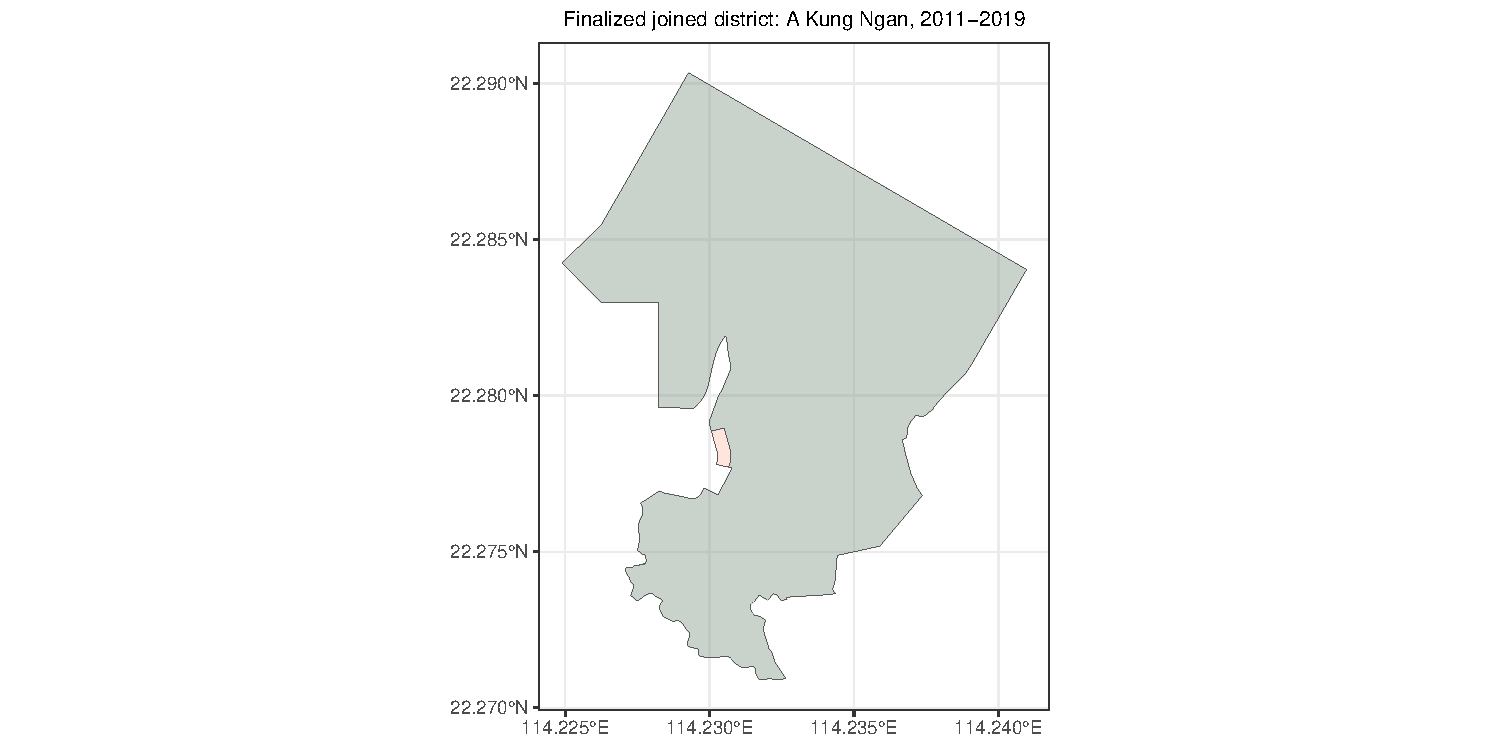
\includegraphics[scale=0.5]{Visuals/joining-district-unchanged.pdf}
        \label{fig: akungngam_joined}
\end{figure}
This figure above shows the geographical areas of an original DCC, A Kung Ngam. This is an example of a district that remained 90 percent unchanged across the three election years. I kept those districts the way they were in the joined district data set.



\subsubsection*{Joined districts}
\begin{figure}[!h]
    \centering
    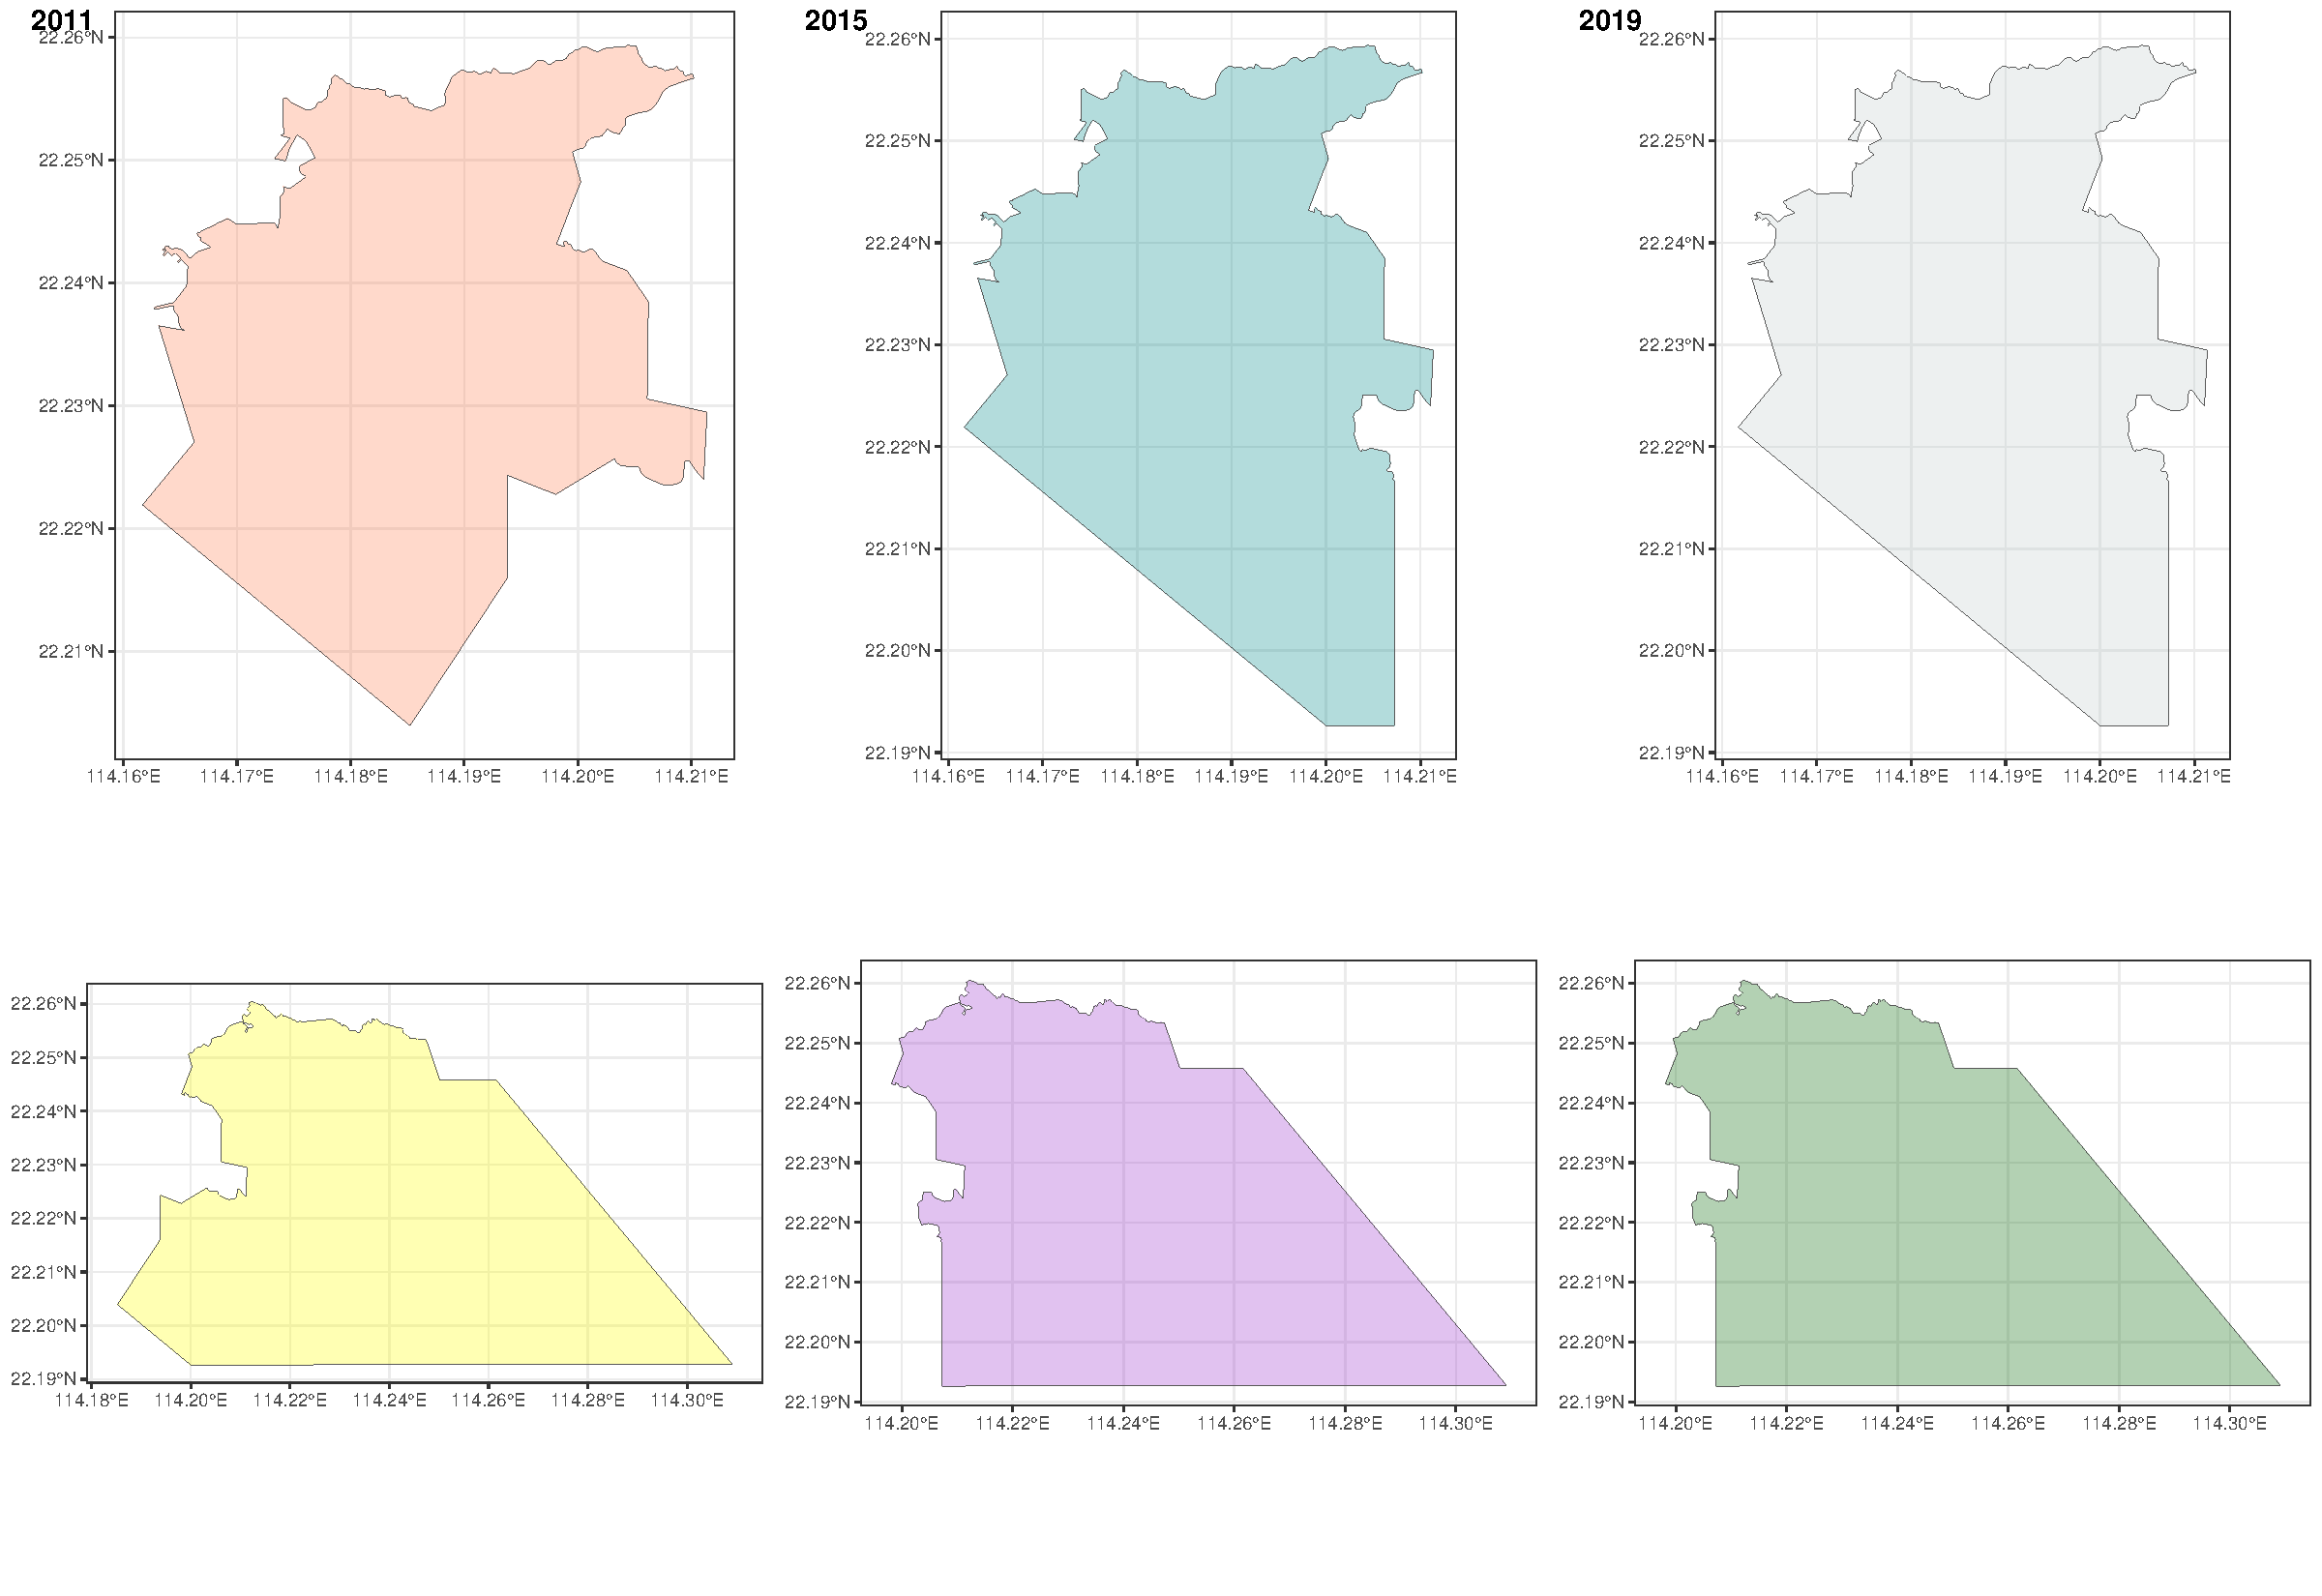
\includegraphics[scale=0.4]{Visuals/changed_joined.pdf}
        \label{joined}
\end{figure}

This figure above shows the geographical areas of two original DCCs. This is an example of a district that did not 90 percent unchanged across the three election years. In this case, changes occurred between 2011 and 2015 as a part of the area in bottom left were drawn into the upper district in the second column in 2015. I combine the two DCCs across three years to ensure that we can observe election outcomes in a stable geographical unit across three years. The finalized district is displayed below.



\begin{figure}[!h]
    \centering
    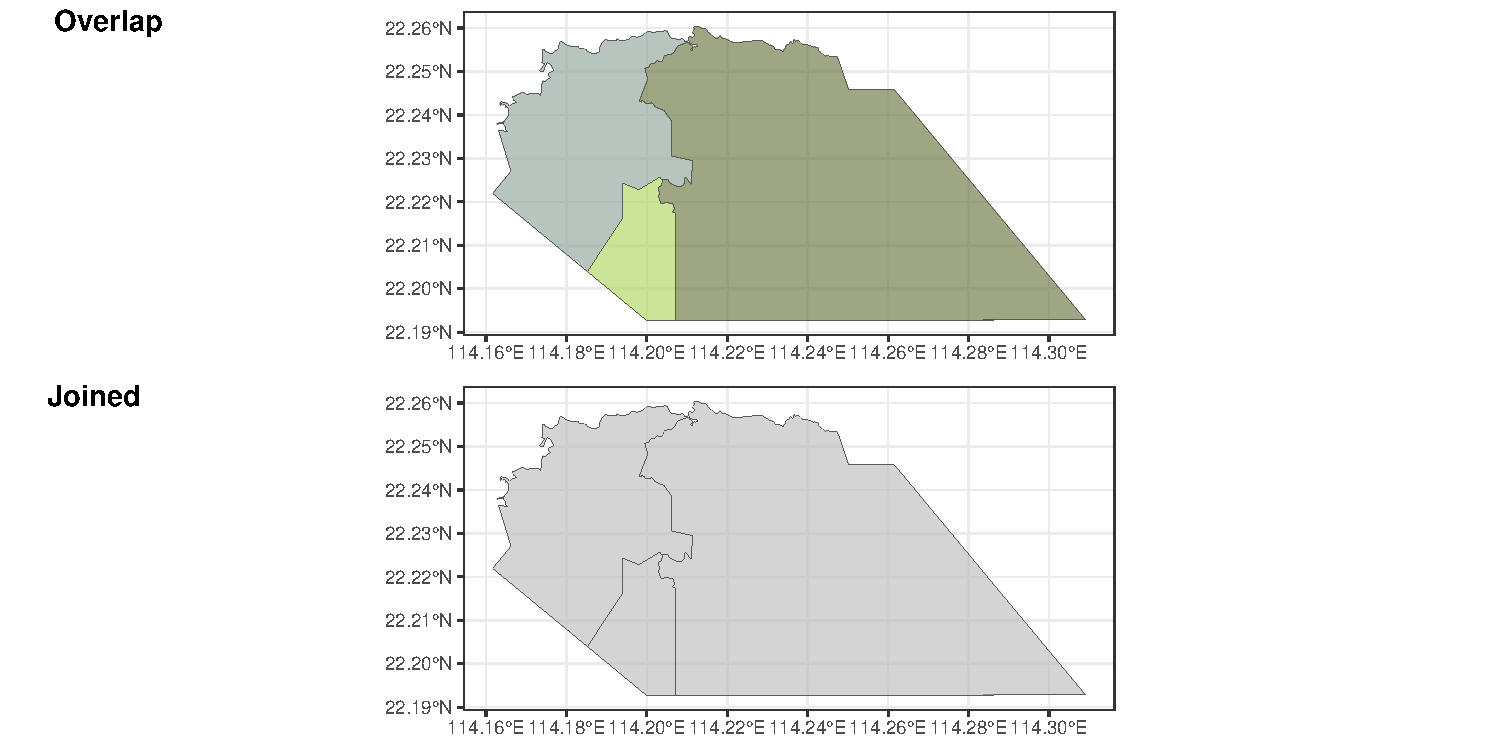
\includegraphics[scale=0.7]{Visuals/combined-final.pdf}
        \label{joined}
\end{figure}

\pagebreak
\section{Replication Package} \label{appendix:replication}
The finalized data frame for analysis and R/Python code used for data collection, cleaning, and visualization in this thesis can be found via my GitHub: \url{https://github.com/jil028/thesis}. Raw full restaurant data are available upon request.

\clearpage
\subsection{Descriptions of Major Variables}
\begingroup
\newcolumntype{C}{>{\RaggedRight\arraybackslash}X}
\begin{table}[h!]
\fontsize{11}{12}\selectfont
\setlength\extrarowheight{3pt} % for a bit of visual "breathing space"
\begin{tabularx}{\textwidth}{CCC}
\toprule
\textbf{Variable Name} & \textbf{Type} & \textbf{Description}  \\
\midrule
\textbf{District FE} & \phantom{} & \phantom{}\\
\midrule
\cellcolor{gray!6}{\texttt{fake\_unit\_id}} & \cellcolor{gray!6}{Character} & \cellcolor{gray!6}{The IDs for joined districts I created as the new unit of analysis to address the issue of redistricting. Districts that remained 90\% unchanged across the three election years are indexed with ``ORIG''.}  \\
\midrule
\textbf{Year FE} & \phantom{} & \phantom{}\\
\midrule
\texttt{year} & Character & The year of the joined district observation. I use data for the District Council Election in 2011, 2015, and 2019.  \\
\midrule
\textbf{Outcomes} & \phantom{} & \phantom{}\\
\midrule
\cellcolor{gray!6}{\texttt{sum\_joined\_dist\_total}} & \cellcolor{gray!6}{Numeric (discrete)} & \cellcolor{gray!6}{The sum of votes cast in a joined district of a given year.}  \\
%\hline
\texttt{prop\_votes\_demo} & Numeric (continuous) & The proportion of votes \n for pro-democracy candidates in \n a joined district of a given year.  \\
%\hline
\cellcolor{gray!6}{\texttt{prop\_votes\_est}} & \cellcolor{gray!6}{Numeric (continuous)} & \cellcolor{gray!6}{The proportion of votes for pro-establishment (pro-Beijing) candidates in a joined district of a given year.}  \\
\midrule
\textbf{Treatment Variables} & \phantom{} & \phantom{}\\
\midrule
\texttt{prop\_Yellow} & Numeric (continuous) & The proportion of ``Yellow'' restaurants in a joined district of a given year.  \\
%\hline
\cellcolor{gray!6}{\texttt{majority\_yellow}} & \cellcolor{gray!6}{Numeric (continuous)} & \cellcolor{gray!6}{Whether the majority of politicized\n restaurants in a joined district of a given year are ``Yellow''. It takes "1" if yes, "0" otherwise.}  \\
\bottomrule
\end{tabularx}
\end{table}
\endgroup{}


\subsection{Data Missingness}
\clearpage
\begin{figure}[!h]
    \centering
    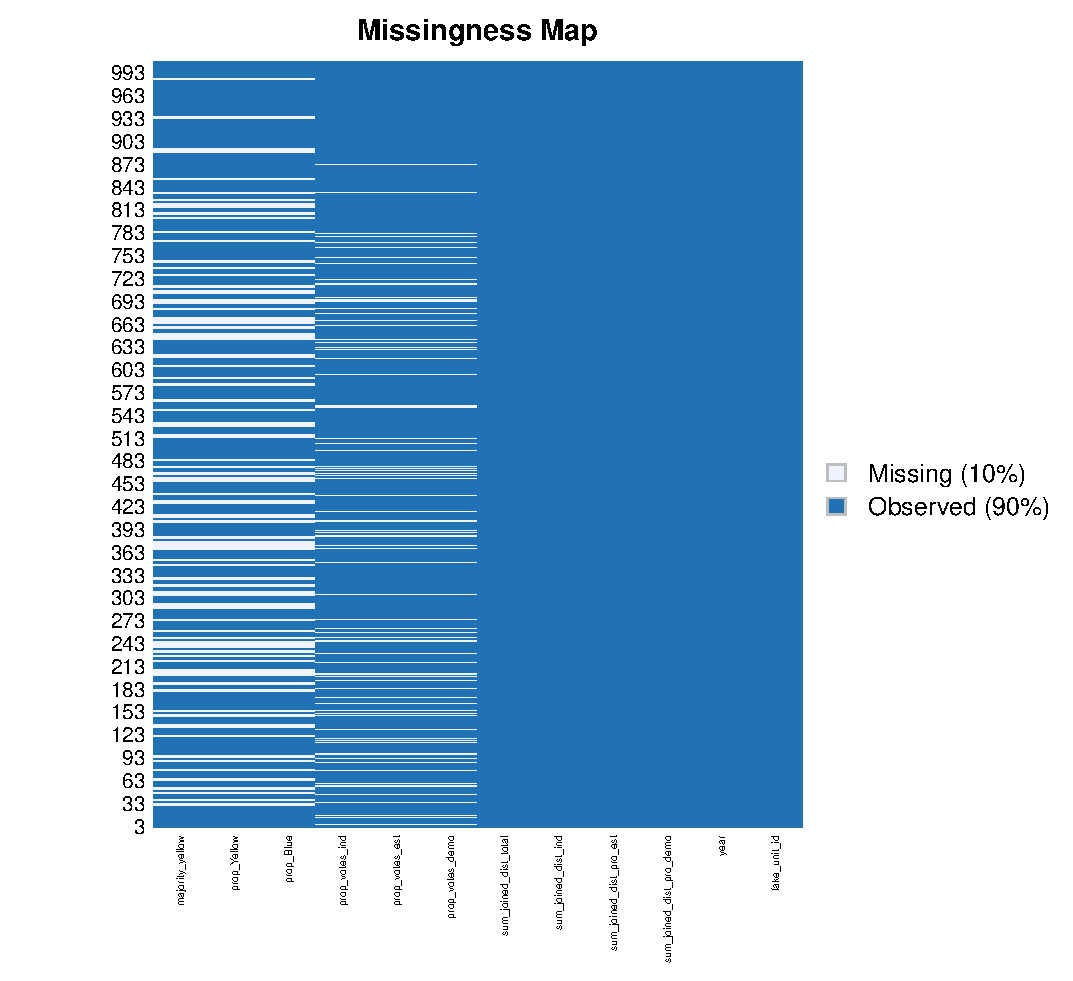
\includegraphics[scale=0.7]{Visuals/missingness.pdf}
    \label{fig:my_label}
\end{figure}








%\pagebreak
\section{Full Restaurant Data} \label{appendix;full_restaurant}

\subsection{Summary Statistics}
\begingroup
\begin{longtable}[c]{lllllll}
\toprule
\textbf{Variable} & \textbf{n} & \textbf{Mean} & \textbf{Std. Dev} & \textbf{Median} & \textbf{Minimum} & \textbf{Maximum}\\
\midrule
\cellcolor{gray!6}{Store Status (binary)} & \cellcolor{gray!6}{4196} & \cellcolor{gray!6}{0.71} & \cellcolor{gray!6}{N/A} & \cellcolor{gray!6}{1.00} & \cellcolor{gray!6}{0} & \cellcolor{gray!6}{1.00}\\
Rating & 4196 & 3.54 & 0.89 & 3.71 & 0 & 4.78\\
\cellcolor{gray!6}{Low Average Price} & \cellcolor{gray!6}{4179} & \cellcolor{gray!6}{75.19} & \cellcolor{gray!6}{51.79} & \cellcolor{gray!6}{51.00} & \cellcolor{gray!6}{50} & \cellcolor{gray!6}{401.00}\\
High Average Price & 2412 & 185.28 & 123.96 & 100.00 & 100 & 800.00\\
\cellcolor{gray!6}{Chain Store (binary)} & \cellcolor{gray!6}{4196} & \cellcolor{gray!6}{0.34} & \cellcolor{gray!6}{N/A} & \cellcolor{gray!6}{0.00} & \cellcolor{gray!6}{0} & \cellcolor{gray!6}{1.00}\\
Political Ideology (binary) & 4196 & 0.46 & N/A & 0.00 & 0 & 1.00\\
\bottomrule
\end{longtable}
\endgroup{}




\subsection{Codeboook}
% table
%\clearpage
\newcolumntype{C}{>{\RaggedRight\arraybackslash}X}
\begin{table}[h!]
\fontsize{11}{12}\selectfont
\setlength\extrarowheight{2pt} % for a bit of visual "breathing space"
\begin{tabularx}{\textwidth}{CCC}
\toprule
\textbf{Variable Name} & \textbf{Type} & \textbf{Description}  \\
\midrule
\cellcolor{gray!6}{\texttt{source}} & \cellcolor{gray!6}{Character (English)} & \cellcolor{gray!6}{The source of data.}  \\
%\hline
\texttt{restaurant\_name} & Character (English and Traditional Chinese) & The name of a restaurant.  \\
%\hline
\cellcolor{gray!6}{\texttt{dce\_constituency}} & \cellcolor{gray!6}{Character (English)} & \cellcolor{gray!6}{The constituency in which the restaurant is located during the 2019 District Council Election}.  \\
%\hline
\texttt{district} & Character (Traditional Chinese) & The district in which the restaurant is located.  \\
%\hline
\cellcolor{gray!6}{\texttt{address}} & \cellcolor{gray!6}{Character (Traditional Chinese)} & \cellcolor{gray!6}{The address of a restaurant.}  \\
%\hline
\texttt{store\_status} & Numeric (binary) & The status of a restaurant (0 = permanently closed; 1 = open).  \\
%\hline
\cellcolor{gray!6}{\texttt{rating}} & \cellcolor{gray!6}{Numeric (continuous)} & \cellcolor{gray!6}{The rating of a restaurant (Possible values: [0, 5]).}  \\
%\hline
\texttt{price} & Character (English and Traditional Chinese) & The average price range for an individual of a restaurant.  \\
%\hline
\cellcolor{gray!6}{\texttt{chain\_store\_indicator}} & \cellcolor{gray!6}{Numeric (binary)} & \cellcolor{gray!6}{Whether there has been more than one restaurant with the same name (0 = only one restaurant; 1 = more than one restaurant).}  \\
%\hline
\texttt{store\_count} & Numeric (discrete) & The number of restaurants with the same name in this data set (Possible Values: \{1, 2, 3, ..., 54, 55\}).  \\
%\hline
\cellcolor{gray!6}{\texttt{ideo\_text}} & \cellcolor{gray!6}{Character (English)} & \cellcolor{gray!6}{Political support of a restaurant (Blue = pro-Beijing; Yellow = pro-democracy).}  \\
%\hline
\texttt{ideo\_bi} & Numeric (binary) & Political support of a restaurant (0 = Blue (pro-Beijing); 1 = Yellow (pro-democracy)).  \\
%\hline
\cellcolor{gray!6}{\texttt{gmaps\_coords}} & \cellcolor{gray!6}{Numeric (continuous)} & \cellcolor{gray!6}{The geographical coordinates (latitude and longitude) of a restaurant retrieved by Google Maps API.}  \\
\bottomrule
\end{tabularx}
%\caption{Codebook of the Restaurant Data Set}
\end{table}



\pagebreak
\clearpage
\section{Audits for Geographic Coordinates} \label{appendix:audits}
Below are results of the audits for geographic coordinates retrieved by Google Maps Geocoding API. I define accuracy as the retrieved coordinates are within 200 meters ($\approx$ 0.12 miles) of the centroid of the actual location of a restaurant. \\
% table
\newcolumntype{C}{>{\RaggedRight\arraybackslash}X}
\begin{table}[h!]
\setlength\extrarowheight{2pt} % for a bit of visual "breathing space"
\begin{tabularx}{\textwidth}{CCCC}
\toprule
\textbf{Data} & \textbf{Audited Sample Size ($\approx 10\%$)} & \textbf{Sample Accuracy Rate} & \textbf{Link}  \\
\midrule
\cellcolor{gray!6}{Restaurants \hphantom{123} ($n = 4196$)} &  \cellcolor{gray!6}{420}  & \cellcolor{gray!6}{95.5\%} & \cellcolor{gray!6}{\href{https://tinyurl.com/2fcfbukr}{tinyurl.com/2fcfbukr}}\\
\bottomrule
\end{tabularx}
\end{table}









\end{appendices}


\end{document}
